%definira klasu dokumenta 
\documentclass[12pt]{report} 

\usepackage[croatian]{babel} 
\usepackage{amssymb}
\usepackage{amsmath}
\usepackage{txfonts}
\usepackage{mathdots}
\usepackage{titlesec}
\usepackage{array}
\usepackage{lastpage}
\usepackage{etoolbox}
\usepackage{tabularray}
\usepackage{color, colortbl}
\usepackage{adjustbox}
\usepackage{geometry}
\usepackage[classicReIm]{kpfonts}
\usepackage{hyperref}
\usepackage{fancyhdr}

\usepackage{float}
\usepackage{setspace}
\restylefloat{table}


\patchcmd{\chapter}{\thispagestyle{plain}}{\thispagestyle{fancy}}{}{} %redefiniranje stila stranice u paketu fancyhdr

%oblik naslova poglavlja
\titleformat{\chapter}{\normalfont\huge\bfseries}{\thechapter.}{20pt}{\Huge}
\titlespacing{\chapter}{0pt}{0pt}{40pt}


\linespread{1.3} %razmak između redaka

\geometry{a4paper, left=1in, top=1in,}  %oblik stranice

\hypersetup{ colorlinks, citecolor=black, filecolor=black, linkcolor=black,	urlcolor=black }   %izgled poveznice


%prored smanjen između redaka u nabrajanjima i popisima
\newenvironment{packed_enum}{
	\begin{enumerate}
		\setlength{\itemsep}{0pt}
		\setlength{\parskip}{0pt}
		\setlength{\parsep}{0pt}
	}{\end{enumerate}}

\newenvironment{packed_item}{
	\begin{itemize}
		\setlength{\itemsep}{0pt}
		\setlength{\parskip}{0pt}
		\setlength{\parsep}{0pt}
	}{\end{itemize}}




%boja za privatni i udaljeni kljuc u tablicama
\definecolor{LightBlue}{rgb}{0.9,0.9,1}
\definecolor{LightGreen}{rgb}{0.9,1,0.9}

%Promjena teksta za dugačke tablice
\DefTblrTemplate{contfoot-text}{normal}{Nastavljeno na idućoj stranici}
\SetTblrTemplate{contfoot-text}{normal}
\DefTblrTemplate{conthead-text}{normal}{(Nastavljeno)}
\SetTblrTemplate{conthead-text}{normal}
\DefTblrTemplate{middlehead,lasthead}{normal}{Nastavljeno od prethodne stranice}
\SetTblrTemplate{middlehead,lasthead}{normal}

%podesavanje zaglavlja i podnožja

\pagestyle{fancy}
\lhead{Programsko inženjerstvo}
\rhead{Štete javnih površina}
\lfoot{CestaFix}
\cfoot{stranica \thepage/\pageref{LastPage}}
\rfoot{\today}
\renewcommand{\headrulewidth}{0.2pt}
\renewcommand{\footrulewidth}{0.2pt}


\begin{document}



\begin{titlepage}
	\begin{center}
		\vspace*{\stretch{1.0}} %u kombinaciji s ostalim \vspace naredbama definira razmak između redaka teksta
		\LARGE Programsko inženjerstvo\\
		\large Ak. god. 2023./2024.\\

		\vspace*{\stretch{3.0}}

		\huge \textbf{Štete javnih površina}\\
		\Large Dokumentacija, Rev. \textit{1}\\

		\vspace*{\stretch{12.0}}
		\normalsize
		Grupa: \textit{CestaFix}\\
		Voditelj: \textit{Fran Fodor}\\


		\vspace*{\stretch{1.0}}
		Datum predaje: \textbf{{17. 11. 2023.}}\\

		\vspace*{\stretch{4.0}}

		Nastavnik: \textit{izv. prof. dr. sc. Vlado Sruk}\\

	\end{center}


\end{titlepage}


\tableofcontents


\chapter{Dnevnik promjena dokumentacije}

\begin{longtblr}[
	label=none
	]{
	width = \textwidth,
	colspec={|X[2]|X[13]|X[5]|X[4]|},
	rowhead = 1
	}
	\hline
	\textbf{Rev.} & \textbf{Opis promjene/dodatka}                                                                                            & \textbf{Autori} & \textbf{Datum} \\[3pt] \hline
	0.1           & Preuzet predložak.                                                                                                        & Sara Podvorec   & 28.10.2023.    \\[3pt] \hline
	0.2           & Dodane osnovne informacije. Napisan početak opisa projekta. Crvenom bojom označeni dijelovi teksta koje treba izmijeniti. & Jan Murić       & 28.10.2023.    \\[3pt] \hline
	0.3           & Nadopuna opisa projekta.                                                                                                  & Sara Podvorec   & 29.10.2023.    \\[3pt] \hline
	0.4           & Nadopuna osnovnih informacija. Nadopuna dnevnika sastajanja.                                                              & Mateo Jakšić    & 30.10.2023.    \\[3pt] \hline
	0.5           & Stiliziranje opisa projekta.                                                                                              & Sara Podvorec   & 30.10.2023.    \\[3pt] \hline
	0.6           & Nadopuna dnevnika sastajanja.                                                                                             & Mateo Jakšić    & 31.10.2023.    \\[3pt] \hline
	0.7           & Nadopuna opisa projektnog zadatka i funkcionalnih zahtjeva.                                                               & Sara Podvorec   & 31.10.2023.    \\[3pt] \hline
	0.8           & Nadopuna literature i funkcionalnih zahtjeva.                                                                             & Mateo Jakšić    & 1.11.2023.     \\[3pt] \hline
	0.9           & Napisan dio obrazaca uporabe                                                                                              & Mateo Jakšić    & 1.11.2023.     \\[3pt] \hline
	0.10          & Nadopuna obrazaca uporabe                                                                                                 & Mateo Jakšić    & 2.11.2023.     \\[3pt] \hline
	0.11          & Nadopuna obrazaca uporabe. Dodani dijagrami obrazaca uporabe.                                                             & Mateo Jakšić    & 6.11.2023.     \\[3pt] \hline
	0.12          & Dodani sekvencijski dijagrami. Dodani ostali zahtjevi. Nadopuna dnevnika sastajanja.                                      & Mateo Jakšić    & 10.11.2023.    \\[3pt] \hline
	0.13          & Dodane osnovne informacije o arhitekturi. Nadopuna opisa baze podataka.                                                   & Sara Podvorec   & 12.11.2023.    \\[3pt] \hline
	0.14          & Dodan opis pojedinih entiteta baze podataka.                                                                              & Sara Podvorec   & 13.11.2023.    \\[3pt] \hline
	0.15          & Nadopuna dnevnika sastajanja. Nadopuna opisa i kreiranje ERD dijagrama baze podataka.                                     & Mateo Jakšić    & 14.11.2023.    \\[3pt] \hline
	0.16          & Dodatan ER dijagram baze podataka                                                                                         & Mateo Jakšić    & 15.11.2023.    \\[3pt] \hline
	0.17          & Dodan opis arhitekture. Dodan vizualni prikaz arhitekture.                                                                & Sara Podvorec   & 16.11.2023.    \\[3pt] \hline
	0.18          & Dodani dijagrami razreda i njihovi opisi. Nadopuna literature.                                                            & Mateo Jakšić    & 16.11.2023.    \\[3pt] \hline
	\textbf{1.0}  & Uklanjanje uputa. Završne nadopune.                                                                                       & Mateo Jakšić    & 17.11.2023.    \\[3pt] \hline
	1.1           & Napisane korištene tehnologije i alati. Nadopunjen dnevnik sastajanja. Prepravljanje osnovnih informacija.                & Mateo Jakšić    & 10.12.2023.    \\[3pt] \hline
	1.2           & Prepravljanje baze podataka.                                                                                              & Mateo Jakšić    & 1.1.2024.      \\[3pt] \hline
	1.3           & Prepravljanje baze podataka i dijagrama razreda.                                                                          & Mateo Jakšić    & 8.1.2024.      \\[3pt] \hline
	1.4           & Dodan dijagram aktivnosti.                                                                                                & Sara Podvorec   & 12.1.2024.     \\[3pt] \hline
	1.5           & Prepravljeni opisi baze podataka i dijagrama razreda.                                                                     & Mateo Jakšić    & 13.1.2024.     \\[3pt] \hline
	1.6           & Dodan dijagram komponentni.                                                                                               & Mateo Jakšić    & 16.1.2024.     \\[3pt] \hline
	1.7           & Dodan prepravljeni dijagram aktivnosti.                                                                                   & Sara Podvorec   & 16.1.2024.     \\[3pt] \hline
	1.8           & Dodan dijagram razmještaja.                                                                                               & Mateo Jakšić    & 16.1.2024.     \\[3pt] \hline
	1.9           & Dodani opisi dijagrama komponenti i dijagrama razmještaja.                                                                & Mateo Jakšić    & 16.1.2024.     \\[3pt] \hline
	1.10          & Dodan dijagram stanja.                                                                                                    & Sara Podvorec   & 17.1.2024.     \\[3pt] \hline
	1.11          & Dodan opis dijagrama stanja i aktivnosti, prepravljen dijagram stanja.                                                    & Sara Podvorec   & 18.1.2024.     \\[3pt] \hline
\end{longtblr}
\chapter{Opis projektnog zadatka}


\textbf{\textit{dio 1. revizije}}\\

{\color{red}\textit{Na osnovi projektnog zadatka detaljno opisati korisničke zahtjeve. Što jasnije opisati cilj projektnog zadatka, razraditi problematiku zadatka, dodati nove aspekte problema i potencijalnih rješenja. Očekuje se minimalno 3, a poželjno 4-5 stranica opisa.	Teme koje treba dodatno razraditi u ovom poglavlju su:}
\begin{packed_item}
	\item \textit{potencijalna korist ovog projekta}
	\item \textit{postojeća slična rješenja (istražiti i ukratko opisati razlike u odnosu na zadani zadatak). Dodajte slike koja predočavaju slična rješenja.}
	\item \textit{skup korisnika koji bi mogao biti zainteresiran za ostvareno rješenje.}
	\item \textit{mogućnost prilagodbe rješenja }
	\item \textit{opseg projektnog zadatka}
	\item \textit{moguće nadogradnje projektnog zadatka}
\end{packed_item}

\textit{Za pomoć pogledati reference navedene u poglavlju „Popis literature“, a po potrebi konzultirati sadržaj na internetu koji nudi dobre smjernice u tom pogledu.}
\eject
}

Svakodnevno se suočavamo s brojnim problemima na javnim površinama i cestama u našim gradovima. Problemi kao što su vandalizam, oštećenje pločnika, udarne rupe na cestama, smeće i slični problemi predstavljaju potencijalnu opasnost za građane te poprilično narušavaju kvalitetu njihovog svakodnevnog života. Neadekvatna briga o oštećenjima i njihovoj sanaciji često ostavlja građane u vrlo nepovoljnoj situaciji kada iste žele prijaviti vlastima.

Kako bi suzbili osjećaj nemoći građana i poboljšali kvalitetu života cjelokupne zajednice, potrebno je omogućiti adekvatnu prijavu oštećenja na javnim površinama.

Glavni cilj ovog projekta je razviti programsku podršku za stvaranje web aplikacije “Unesi ime aplikacije koje moramo smisliti” za dojavu oštećenja i drugih problema na cestama, parkovima, javnim ustanovama i ostalim javnim mjestima u svrhu olakšavanja dojave, kategorizacije te u konačnici rješenja prijavljenih problema.

Ideja je omogućiti građanima da na što jednostavniji način prijavljuju oštećenja i probleme na javnim površinama i cestama svojih gradova te tako pomognu lokalnim vlastima da pravodobno reagiraju na nastale probleme. S obzirom na velik broj javih ustanova i njihovih odjeljaka koji se bave različitim problemima, teško je pratiti tko je nadležan za koju vrstu problema i nad kojim područjem. Sustav bi automatski odredio nadležno tijelo prema kategoriji prijave i drugim parametrima te proslijedio prijavu na obradu. Ključno je da proces prijave bude jednostavan i brz.

Prilikom pokretanja sustava prikazuje se početna stranica na kojoj se nalazi karta sa označenim lokacijama već podnesenih prijava raznovrsnih oštećenja javnih površina, nekoliko informacija o samoj aplikaciji te navigacijski izbornik putem kojeg se pristupa registraciji/prijavi u sustav te podnošenju prijava i provjeri statusa već podnesenih prijava.

Svakom neregistriranom korisniku omogućeno je prijavljivanje u sustav s postojećim računom, prilikom čega je potrebno upisati korisničko ime i lozinku, ili kreiranje novog računa prilikom čega je potrebno odabrati korisničko ime i lozinku te upisati valjanu email adresu.

Također, postoji opcija anonimnog podnošenja prijave na temelju koje se status podnesene prijave prati putem jedinstvenog broja prijave bez iznošenja osobnih podataka.

Registrirani korisnik može pregledavati i mijenjati svoje osobne podatke i izbrisati svoj korisnički račun te postoji mogućnost naknadne dodjele prava službenika ili administratora stupanjem u kontakt naveden pri dnu stranice.

Kako bi olakšala proces podnošenja prijave, aplikacija omogućuje građanima da brzo i precizno dokumentiraju probleme. Svaka prijava uključuje naziv problema, kratki opis, geografske koordinate problema, jedinstveni broj prijave te opcionalno fotografije kako bi se problem što bolje opisao. Građani mogu odabirom lokacije na karti, unosom najbliže adrese ili iz meta podataka slika priloženih uz prijavu precizno definirati lokaciju problema na koji su naišli.

Sustav također olakšava identifikaciju vremenski bliskih prijava na istoj lokaciji kako bi se građani mogli povezati na već postojeće prijave sličnih problema, čime se smanjuje dupliciranje prijava i ubrzava proces njihovog rješavanja.

Podnesene prijave obrađuju određeni gradski uredi, a svaka promjena u statusu prijave vidljiva je prijavitelju i svim ostalim korisnicima koji su povezani s tom lokacijom. Gradski uredi također imaju mogućnost objediniti nepovezane prijave na istoj lokaciji, što je vidljivo prijaviteljima.

Kako bi gradskim uredima olakšali razvrstavanje i obrađivanje prijava, sustav dopušta prijave za različite kategorije problema.

Sve podnesene prijave su javno dostupne i mogu se grupirati prema temi i lokaciji, što omogućuje građanima i vlastima da prate i analiziraju probleme u stvarnom vremenu.

Korisnik s pravom službenika ima mogućnost ažuriranja statusa prijava i pregled profila prijavitelja (ili jedinstvenog broja prijave u slučaju anonimnog prijavitelja) među kojima odabire relevantne prijave. Nakon što sustav proslijedi prijavu u nadležni gradski ured, službenik tog ureda može izabrati problem i krenuti raditi na njegovu rješenju.

Administrator sustava ima najveće ovlasti među koje pripada i pristup bazi s popisom registriranih korisnika i njihovim podacima te mogućnost brisanja korisnika kao i dodjeljivanje administratorskih prava i prava službenika drugim korisnicima.

Statistika o statusima prijava, poput vremena potrebnog za rješavanje problema, također se obrađuje u stvarnom vremenu kako bi poboljšala učinkovitost sustava.

Posebna je pozornost posvećena zaštiti svih osobnih podataka te osiguranju korisničkog iskustva koje će biti jednostavno i intuitivno, kako bi se potaknulo građane na aktivno sudjelovanje u poboljšanju svojih zajednica.

Jedan od primjera sličnog sustava koji se aktivno upotrebljava u Hrvatskoj je "Gradsko Oko". Projekt je pokrenut u kolovozu 2017. godine u svrhu prijave komunalnih problema na području grada Bjelovara, a od tad se proširio na još 11 gradova i općina te na prijavu problema na moru.

Iako je projekt sličan našem razlikuje se u nekoliko točaka: ne dozvoljava anonimne prijave, ne sadrži mogućnost pregleda statistike i ne provjerava sličnost vremenski bliskih prijava u svrhu grupiranja.




\chapter{Specifikacija programske potpore}

\section{Funkcionalni zahtjevi}

\noindent \textbf{Dionici:}

\begin{packed_enum}

	\item Neregistrirani korisnik
	\item Registrirani korisnik
	\begin{packed_enum}
		\item Građanin
		\item Službenik gradskog ureda
	\end{packed_enum}
	\item Administrator
	\item Razvojni tim
	\item Suradnici
	\begin{packed_enum}
		\item Nastavnik
		\item Demonstrator
	\end{packed_enum}

\end{packed_enum}

\noindent \textbf{Aktori i njihovi funkcionalni zahtjevi:}


\begin{packed_enum}
	\item  \underbar{Neregistrirani korisnik (inicijator) može:}

	\begin{packed_enum}

		\item podnositi anonimne prijave
		\item pratiti status prijave jedinstvenim brojem prijave
		\item imati uvid u postojeće prijave
		\item imati uvid u statistiku statusa prijava
		\item registrirati korisnički račun


	\end{packed_enum}

	\item  \underbar{Građanin (inicijator) može:}

	\begin{packed_enum}

		\item prijaviti se na korisnički račun
		\item odjaviti se s korisničkog računa
		\item pratiti status vlastitih prijava
		\item imati uvid u postojeće prijave
		\item imati uvid u statistiku statusa prijava
		\item izmijeniti podatke korisničkog računa

	\end{packed_enum}

	\item \underbar{Službenik gradskog ureda (inicijator) može:}

	\begin{packed_enum}

		\item obrađivati podnesene prijave
		\item objediniti nepovezane prijave po temi i lokaciji
		\item promijeniti status prijave
		\item pratiti i analizirati probleme u stvarnom vremenu
		\item izmijeniti podatke korisničkog računa

	\end{packed_enum}

	\item \underbar{Administrator (inicijator) može:}

	\begin{packed_enum}

		\item uređivati i brisati korisničke račune
		\item pristupiti bazi podataka
		\item kreirati i ukloniti gradski ured
		\item dodijeliti i ukloniti ulogu službenika gradskog ureda registriranom korisniku 
		\item dodijeliti i ukloniti ulogu administratora registriranom korisniku 
	\end{packed_enum}

	\item \underbar{Baza podataka (sudionik) može:}

	\begin{packed_enum}

		\item pohraniti sve podatke o korisnicima i njihovim ulogama
		\item pohraniti sve podatke o prijavljenim oštećenjima
		\item pohraniti sve podatke o kategorijama problema i gradskim uredima za njihovo obrađivanje

	\end{packed_enum}

\end{packed_enum}


\eject



\subsection{Obrasci uporabe}

\subsubsection{Opis obrazaca uporabe}

\noindent \underbar{\textbf{UC01 - Registracija korisničkog računa}}
\begin{packed_item}

	\item \textbf{Glavni sudionik: }Neregistrirani korisnik
	\item  \textbf{Cilj:} Stvaranje korisničkog račun za pristup sustavu
	\item  \textbf{Sudionici:} Baza podataka
	\item  \textbf{Preduvjet:} -
	\item  \textbf{Opis osnovnog tijeka:}

	\item[] \begin{packed_enum}

		\item Korisnik odabire opciju za prijavu
		\item Korisnik odabire opciju da nema korisnički račun
		\item Korisnik unosi potrebne podatke i potvrđuje unos
		\item Korisnik se upisuje u bazu podataka i korisnik se preusmjerava na početnu stranicu
	\end{packed_enum}

	\item  \textbf{Opis mogućih odstupanja:}

	\item[] \begin{packed_item}

		\item[3.a] Odabir već zauzetog korisničkog imena i/ili e-mail adrese, unos korisničkih podataka u neispravnom formatu, nepodudaranje lozinki
		\item[] \begin{packed_enum}

			\item Sustav obavještava korisnika o neuspjelom unosu i vraća ga na stranicu za registraciju
			\item Korisnik mijenja potrebne podatke te završava unos ili odustaje od registracije

		\end{packed_enum}
	\end{packed_item}
\end{packed_item}

\noindent \underbar{\textbf{UC02 - Prijava na korisnički račun}}
\begin{packed_item}

	\item \textbf{Glavni sudionik: }Registrirani korisnik
	\item  \textbf{Cilj:} Dobivanje pristupa korisničkom sučelju s ovlastima registriranog korisnika
	\item  \textbf{Sudionici:} Baza podataka
	\item  \textbf{Preduvjet:} Korisnik je obavio registraciju i njegovi podaci se nalaze u bazi podataka
	\item  \textbf{Opis osnovnog tijeka:}

	\item[] \begin{packed_enum}

		\item Korisnik odabire opciju za prijavu
		\item Korisnik unosi korisničko ime i lozinku te potvrđuje unos
		\item Korisnik se preusmjerava na početnu stranicu
	\end{packed_enum}

	\item  \textbf{Opis mogućih odstupanja:}

	\item[] \begin{packed_item}

		\item[2.a] Neispravni unos korisničkog imena i/ili lozinke
		\item[] \begin{packed_enum}

			\item Sustav obavještava korisnika o neuspjelom unosu i vraća ga na stranicu za prijavu
			\item Korisnik unosi ispravne podatke te završava unos ili odustaje od prijave

		\end{packed_enum}
	\end{packed_item}
\end{packed_item}

\noindent \underbar{\textbf{UC03 - Odjava s korisničkog računa}}
\begin{packed_item}

	\item \textbf{Glavni sudionik: }Registrirani korisnik
	\item  \textbf{Cilj:} Izlazak iz korisničkog sučelja
	\item  \textbf{Sudionici:} Baza podataka
	\item  \textbf{Preduvjet:} Korisnik je obavio prijavu na korisnički račun
	\item  \textbf{Opis osnovnog tijeka:}

	\item[] \begin{packed_enum}

		\item Korisnik odabire opciju za odjavu
		\item Korisnik se preusmjerava na početnu stranicu
	\end{packed_enum}
\end{packed_item}


\noindent \underbar{\textbf{UC04 - Kreiranje gradskog ureda}}
\begin{packed_item}

	\item \textbf{Glavni sudionik: }Administratori
	\item  \textbf{Cilj:} Kreiranje gradskog ureda
	\item  \textbf{Sudionici:} Baza podataka
	\item  \textbf{Preduvjet:} Korisnik je prijavljen i ima administrator ovlasti
	\item  \textbf{Opis osnovnog tijeka:}

	\item[] \begin{packed_enum}

		\item Korisnik otvara padajući izbornik
		\item Korisnik odabire opciju za kreiranje gradskog ureda
		\item Korisnik unosi potrebne podatke i potvrđuje unos
		\item Gradski ured se upisuje u bazu podataka i korisnik se preusmjerava na početnu stranicu

	\end{packed_enum}

	\item  \textbf{Opis mogućih odstupanja:}

	\item[] \begin{packed_item}

		\item[3.a] Odabir već zauzetog imena gradskog ureda
		\item[] \begin{packed_enum}

			\item Sustav obavještava korisnika o neuspjelom unosu i vraća ga na stranicu za kreiranje gradskog ureda
			\item Korisnik mijenja potrebne podatke te završava unos ili odustaje od kreiranja gradskog ureda

		\end{packed_enum}
		\item[3.b] Nije odabrana nijedna kategorija oštećenja kojom će gradski ured upravljati
		\item[] \begin{packed_enum}

			\item Sustav obavještava korisnika o obveznom unosu barem jedne kategorije oštećenja kojom će ured upravljati
			\item Korisnik odabire barem jednu kategoriju oštećenja te završava unos ili odustaje od kreiranja gradskog ureda

		\end{packed_enum}

	\end{packed_item}
\end{packed_item}


\noindent \underbar{\textbf{UC05 - Uklanjanje gradskog ureda}}
\begin{packed_item}

	\item \textbf{Glavni sudionik: }Administrator
	\item  \textbf{Cilj:} Uklanjanje gradskog ureda
	\item  \textbf{Sudionici:} Baza podataka
	\item  \textbf{Preduvjet:} Korisnik je prijavljen i ima administrator ovlasti, gradski ured postoji
	\item  \textbf{Opis osnovnog tijeka:}

	\item[] \begin{packed_enum}

		\item Korisnik otvara padajući izbornik
		\item Korisnik odabire opciju za pregled gradskih ureda
		\item Korisnik odabire gradski ured
		\item Korisnik odabire opciju za uklanjanje gradskog ureda 
		\item Gradski ured se uklanja iz baze podataka i korisnik se preusmjerava na stranicu za pregled gradskih ureda
	\end{packed_enum}
\end{packed_item}


\noindent \underbar{\textbf{UC06 - Dodjela uloge službenika gradskog ureda}}
\begin{packed_item}

	\item \textbf{Glavni sudionik: }Administrator
	\item  \textbf{Cilj:} Dodjeljivanje uloge službenika gradskog ureda registriranom korisniku
	\item  \textbf{Sudionici:} Baza podataka
	\item  \textbf{Preduvjet:} Korisnik je prijavljen i ima administratorske ovlasti, postoji odgovarajući gradski ured za registriranog korisnika
	\item  \textbf{Opis osnovnog tijeka:}

	\item[] \begin{packed_enum}

		\item Korisnik otvara padajući izbornik 
		\item Korisnik odabire opciju za pregled popisa korisničkih računa
		\item Korisnik odabire korisnički račun
		\item Korisnik odabire opciju za dodjelu uloge službenika gradskog ureda
		\item Registrirani korisnik dobiva ulogu službenika gradskog ureda i korisnik se preusmjerava na pregled korisničkog računa
	\end{packed_enum}
\end{packed_item}


\noindent \underbar{\textbf{UC07 - Pregled korisničkog računa}}
\begin{packed_item}

	\item \textbf{Glavni sudionik: }Registrirani korisnik
	\item  \textbf{Cilj:} Pregledavanje korisničkog račun
	\item  \textbf{Sudionici:} Baza podataka
	\item  \textbf{Preduvjet:} Korisnik je obavio prijavu na korisnički račun
	\item  \textbf{Opis osnovnog tijeka:}

	\item[] \begin{packed_enum}

		\item Korisnik otvara padajući izbornik
		\item Korisnik odabire opciju za pregled vlastitog korisničkog računa
	\end{packed_enum}
\end{packed_item}


\noindent \underbar{\textbf{UC08 - Uređivanje podataka korisničkog računa}}
\begin{packed_item}

	\item \textbf{Glavni sudionik: }Registrirani korisnik
	\item  \textbf{Cilj:} Promjena podataka na vlastitom korisničkom računu 
	\item  \textbf{Sudionici:} Baza podataka
	\item  \textbf{Preduvjet:} Korisnik je obavio prijavu na korisnički račun
	\item  \textbf{Opis osnovnog tijeka:}

	\item[] \begin{packed_enum}

		\item Korisnik otvara padajući izbornik
		\item Korisnik odabire opciju za pregled vlastitog korisničkog računa
		\item Korisnik odabire opciju za uređivanje korisničkih podataka
		\item Korisnik uređuje korisničke podatke i potvrđuje promjene
		\item Korisnički podaci se ažuriraju u bazi podataka i korisnik se preusmjerava na pregled vlastitog korisničkog računa
	\end{packed_enum}

	\item  \textbf{Opis mogućih odstupanja:}

	\item[] \begin{packed_item}

		\item[4.a] Odabir već zauzetog korisničkog imena i/ili e-mail adrese, unos korisničkog podatka u neispravnom formatu, nepodudaranje lozinki
		\item[] \begin{packed_enum}

			\item Sustav obavještava korisnika o neuspjelom unosu i vraća ga na uređivanje korisničkih podataka
			\item Korisnik mijenja potrebne podatke te završava unos ili odustaje od uređivanja korisničkih podataka

		\end{packed_enum}
	\end{packed_item}
\end{packed_item}


\noindent \underbar{\textbf{UC09 - Brisanje korisničkog računa}}
\begin{packed_item}

	\item \textbf{Glavni sudionik: }Registrirani korisnik
	\item  \textbf{Cilj:} Uklanjanje vlastitog korisničkog računa
	\item  \textbf{Sudionici:} Baza podataka
	\item  \textbf{Preduvjet:} Korisnik je obavio prijavu na korisnički račun
	\item  \textbf{Opis osnovnog tijeka:}

	\item[] \begin{packed_enum}

		\item Korisnik otvara padajući izbornik
		\item Korisnik odabire opciju za pregled vlastitog korisničkog računa
		\item Korisnik odabire opciju za brisanje korisničkog računa
		\item Korisnik povrđuje odluku i korisnik se preusmjerava na početnu stranicu
	\end{packed_enum}
\end{packed_item}


\noindent \underbar{\textbf{UC10 - Kreiranje anonimne prijave oštećenja}}
\begin{packed_item}

	\item \textbf{Glavni sudionik: }Neregistrirani korisnik
	\item  \textbf{Cilj:} Prijava oštećenja
	\item  \textbf{Sudionici:} Baza podataka
	\item  \textbf{Preduvjet:} -
	\item  \textbf{Opis osnovnog tijeka:}

	\item[] \begin{packed_enum}

		\item Korisnik odabire opciju za prijavu oštećenja
		\item Korisnik unosi potrebne podatke i potvrđuje unos
		\item Prijava oštećenja se upisuje u bazu podataka i korisnik dobiva jedinstveni broj prijave
	\end{packed_enum}

	\item  \textbf{Opis mogućih odstupanja:}

	\item[] \begin{packed_item}

		\item[2.a] Neuneseni obvezni podaci i/ili podaci uneseni u neispravnom formatu 
		\item[] \begin{packed_enum}

			\item Sustav obavještava korisnika o neuspjelom unosu i vraća ga na stranicu za prijavu oštećenja
			\item Korisnik mijenja potrebne podatke te završava unos ili odustaje od prijave oštećenja

		\end{packed_enum}
	\end{packed_item}
\end{packed_item}


\noindent \underbar{\textbf{UC11 - Kreiranje prijave oštećenja}}
\begin{packed_item}

	\item \textbf{Glavni sudionik: }Registrirani korisnik
	\item  \textbf{Cilj:} Prijava oštećenja
	\item  \textbf{Sudionici:} Baza podataka
	\item  \textbf{Preduvjet:} Korisnik je prijavljen
	\item  \textbf{Opis osnovnog tijeka:}

	\item[] \begin{packed_enum}

		\item Korisnik odabire opciju za prijavu oštećenja
		\item Korisnik unosi potrebne podatke i potvrđuje unos
		\item Prijava oštećenja se upisuje u bazu podataka i korisnik se preusmjerava na početnu stranicu
	\end{packed_enum}

	\item  \textbf{Opis mogućih odstupanja:}

	\item[] \begin{packed_item}

		\item[2.a] Neuneseni obvezni podaci i/ili podaci uneseni u neispravnom formatu 
		\item[] \begin{packed_enum}

			\item Sustav obavještava korisnika o neuspjelom unosu i vraća ga na stranicu za prijavu oštećenja
			\item Korisnik mijenja potrebne podatke te završava unos ili odustaje od prijave oštećenja

		\end{packed_enum}
	\end{packed_item}
\end{packed_item}


\noindent \underbar{\textbf{UC12 - Provjera statusa anonimne prijave oštećenja}}
\begin{packed_item}

	\item \textbf{Glavni sudionik: } Neregistrirani korisnik
	\item  \textbf{Cilj:} Provjera statusa anonimne prijave oštećenja
	\item  \textbf{Sudionici:} Baza podataka
	\item  \textbf{Preduvjet:} Podnesena prijava oštećenja
	\item  \textbf{Opis osnovnog tijeka:}

	\item[] \begin{packed_enum}

		\item Korisnik odabire opciju za provjeru statusa prijave oštećenja
		\item Korisnik unosi jedinstveni broj prijave i potvrđuje unos
	\end{packed_enum}

	\item  \textbf{Opis mogućih odstupanja:}

	\item[] \begin{packed_item}

		\item[2.a] Jedinstveni broj prijave ne postoji ili je unesen u neispravnom formatu
		\item[] \begin{packed_enum}

			\item Sustav obavještava korisnika o neuspjelom unosu i vraća ga na stranicu za provjeru statusa prijave oštećenja
			\item Korisnik unosi ispravni jedinstveni broj prijave i završava unos ili odustaje od provjere statusa prijave oštećenja

		\end{packed_enum}

	\end{packed_item}
\end{packed_item}


\noindent \underbar{\textbf{UC13 - Provjera statusa prijave oštećenja}}
\begin{packed_item}

	\item \textbf{Glavni sudionik: } Registrirani korisnik
	\item  \textbf{Cilj:} Provjera statusa vlastite prijave oštećenja
	\item  \textbf{Sudionici:} Baza podataka
	\item  \textbf{Preduvjet:} Podnesena prijava oštećenja, korisnik je prijavljen
	\item  \textbf{Opis osnovnog tijeka:}

	\item[] \begin{packed_enum}

		\item Korisnik odabire opciju za provjeru statusa prijave oštećenja
		\item Korisnik odabire prijavu oštećenja za koju želi provjeriti status oštećenja
	\end{packed_enum}
\end{packed_item}


\noindent \underbar{\textbf{UC14 - Pregled prijave oštećenja}}
\begin{packed_item}

	\item \textbf{Glavni sudionici: } Registrirani korisnik, Neregistrirani korisnik
	\item  \textbf{Cilj:} Pregled prijave oštećenja
	\item  \textbf{Sudionici:} Baza podataka
	\item  \textbf{Preduvjet:} -
	\item  \textbf{Opis osnovnog tijeka:}

	\item[] \begin{packed_enum}

		\item Pregled prijave oštećenja
		\item Korisniku se otvara pregled prijavljeno oštećenje 
	\end{packed_enum}
\end{packed_item}


\noindent \underbar{\textbf{UC15 - Promjena statusa prijave oštećenja}}
\begin{packed_item}

	\item \textbf{Glavni sudionik: }Službenik gradskog ureda
	\item  \textbf{Cilj:} Promjena statusa prijave oštećenja
	\item  \textbf{Sudionici:} Baza podataka
	\item  \textbf{Preduvjet:} Podnesena prijava oštećenja, korisnik ima ulogu službenika gradskog ureda
	\item  \textbf{Opis osnovnog tijeka:}

	\item[] \begin{packed_enum}

		\item Korisnik odabire opciju za prikaz popisa prijavljenih oštećenja
		\item Korisnik odabire prijavu oštećenja
		\item Korisnik odabire opciju za promjenu statusa prijave i potvrđuje promjenu
		\item Status prijave oštećenja se ažurira u bazi podataka i korisnik se preusmjerava na pregled prijave oštećenja
	\end{packed_enum}
\end{packed_item}


\noindent \underbar{\textbf{UC16 - Provjera statistike statusa prijave oštećenja}}
\begin{packed_item}

	\item \textbf{Glavni sudionici: } Neregistrirani korisnik, Registrirani korisnik
	\item  \textbf{Cilj:} Provjera statistike statusa prijave oštećenja
	\item  \textbf{Sudionici:} Baza podataka
	\item  \textbf{Preduvjet:} -
	\item  \textbf{Opis osnovnog tijeka:}

	\item[] \begin{packed_enum}

		\item Korisnik odabire opciju za provjeru statistike statusa prijava oštećenja
		\item Korisniku se otvara pregled statistike statusa prijava oštećenja
	\end{packed_enum}
\end{packed_item}


\noindent \underbar{\textbf{UC17 - Objedinjavanje nepovezanih prijava oštećenja}}
\begin{packed_item}

	\item \textbf{Glavni sudionik: } Službenik gradskog ureda
	\item  \textbf{Cilj:} Objediniti nepovezane prijave oštećenja po temi i lokaciji
	\item  \textbf{Sudionici:} Baza podataka
	\item  \textbf{Preduvjet:} Postoje prijave oštećenja s istom temom i lokacijom, korisnik ima ulogu službenika gradskog ureda
	\item  \textbf{Opis osnovnog tijeka:}

	\item[] \begin{packed_enum}

		\item Korisnik odabire opciju za prikaz popisa prijavljenih oštećenja
		\item Korisnik odabire opciju za objedinjavanje prijava oštećenja
		\item Korisnik odabire dvije ili više prijava oštećenja i potvrđuje odabir
		\item Prijave oštećenja se objedinjuju u bazi podataka i korisnik se preusmjerava na početnu stranicu
	\end{packed_enum}

	\item  \textbf{Opis mogućih odstupanja:}

	\item[] \begin{packed_item}

		\item[3.a] Korisnik je odabrao manje od dvije prijave oštećenja i pokušao napraviti objedinjavanje
		\item[] \begin{packed_enum}

			\item Sustav obavještava korisnika o neuspjelom pokušaju objedinjavanja i vraća ga na odabir prijava oštećenja
			\item Korisnik odabire više od dvije prijave oštećenja i potvrđuje odabir ili odustaje od objedinjavanja prijava oštećenja
		\end{packed_enum}

	\end{packed_item}
\end{packed_item}


\noindent \underbar{\textbf{UC18 - Dodjela kategorije za upravljanje gradskom uredu}}
\begin{packed_item}

	\item \textbf{Glavni sudionik: }Administrator
	\item  \textbf{Cilj:} Dodjela kategorije oštećenja kojom će određeni gradski ured upravljati
	\item  \textbf{Sudionici:} Baza podataka
	\item  \textbf{Preduvjet:} Gradski ured postoji, korisnik ima ulogu administratora
	\item  \textbf{Opis osnovnog tijeka:}

	\item[] \begin{packed_enum}

		\item Korisnik odabire padajući izbornik
		\item Korisnik odabire opciju pregleda gradskih ureda
		\item Korisnik odabire gradski ured
		\item Korisnik odabire opciju za dodavanje kategorija oštećenja 
		\item Korisnik radi odabir kategorija i potvđuje odabir
		\item Ažurirani popis kategorija oštećenja za koje je zadužen gradski ured se upisuje u bazu podataka i korisnik se preusmjerava na pregled profila gradskog ureda
	\end{packed_enum}

	\item  \textbf{Opis mogućih odstupanja:}

	\item[] \begin{packed_item}

		\item[4.a] Gradski ured već upravlja svim kategorijama oštećenja, ne postoji kategorija oštećenja kojom već ne upravlja neki gradski ured u istom mjestu
		\item[] \begin{packed_enum}

			\item Sustav obavještava korisnika da ne postoji kategorija oštećenja kojom gradski ured već ne upravlja ili da ne postoji kategorija kojom već ne upravlja neki gradski ured u istom mjestu
			\item Korisnik odustaje od dodjele kategorije za upravljanje gradskom uredu

		\end{packed_enum}
	\end{packed_item}
\end{packed_item}


\noindent \underbar{\textbf{UC19 - Uklanjanje kategorije za upravljanje iz gradskog ureda}}
\begin{packed_item}

	\item \textbf{Glavni sudionik: }Administrator
	\item  \textbf{Cilj:} Uklanjanje kategorije oštećenja kojom trenutno upravlja gradski ured
	\item  \textbf{Sudionici:} Baza podataka
	\item  \textbf{Preduvjet:} Gradski ured postoji, korisnik ima ulogu administratora
	\item  \textbf{Opis osnovnog tijeka:}

	\item[] \begin{packed_enum}

		\item Korisnik odabire padajući izbornik
		\item Korisnik odabire opciju pregleda gradskih ureda
		\item Korisnik odabire gradski ured
		\item Korisnik odabire opciju da uklanjanje kategorija oštećenja
		\item Korisnik radi odabir kategorija i potvđuje ga
		\item Ažurirani popis kategorija oštećenja za koje je zadužen gradski ured se upisuje u bazu podataka i korisnik se preusmjerava na pregled profila gradskog ureda
	\end{packed_enum}

	\item  \textbf{Opis mogućih odstupanja:}

	\item[] \begin{packed_item}

		\item[5.a] Korisnik je odabrao sve kategorije oštećenja 
		\item[] \begin{packed_enum}

			\item Sustav obavještava korisnika da je odabrao sve kategorije oštećenja i vraća ga na stranicu za uređivanje gradskog ureda s otvorenom opcijom odabira kategorija
			\item Korisnik odabire kategorije pazeći da ostavi barem jednu kategoriju i potvrđuje odabir ili odustaje od uklanjanja kategorija oštećenja kojima upravlja gradski ured

		\end{packed_enum}
	\end{packed_item}
\end{packed_item}


\noindent \underbar{\textbf{UC20 - Ponovno postavljanje zaboravljene lozinke}}
\begin{packed_item}

	\item \textbf{Glavni sudionik: }Registrirani korisnik
	\item  \textbf{Cilj:} Stvaranje nove lozinke za registriranog korisnika
	\item  \textbf{Sudionici:} Baza podataka
	\item  \textbf{Preduvjet:} Korisnik je registriran i njegovi podaci se nalaze u bazi podataka
	\item  \textbf{Opis osnovnog tijeka:}

	\item[] \begin{packed_enum}

		\item Korisnik odabire opciju za prijavu
		\item Korisnik odabire opciju za ponovno postavljanje zaboravljene lozinke
		\item Korisnik unosi e-mail adresu korisničkog računa i potvrđuje unos
		\item Korisnik dobiva personalizirani link na stranicu gdje mijenja lozinku
		\item Korisnik unosi novu lozinku i potvrđuje odabir
		\item Nova lozinka sprema se u bazu podataka i korisnik se preusmjerava na početnu stranicu
	\end{packed_enum}

	\item  \textbf{Opis mogućih odstupanja:}

	\item[] \begin{packed_item}

		\item[3.a] Unesena e-mail adresa ne postoji ili je u neispravnom formatu
		\item[] \begin{packed_enum}

			\item Sustav obavještava korisnika da e-mail adresa ne postoji ili je u neispravnom formatu
			\item Korisnik unosi ispravnu e-mail adresu ili odustaje od ponovnog postavljanja zaboravljene lozinke

		\end{packed_enum}
		\item[4.a] Uneseni identifikacijski broj ne postoji ili je u neispravnom formatu
		\item[] \begin{packed_enum}

			\item Sustav obavještava korisnika da identifikacijski broj ne postoji ili je u neispravnom formatu
			\item Korisnik unosi ispravni identifikacijski broj ili odustaje od ponovnog postavljanja zaboravljene lozinke

		\end{packed_enum}
		\item[5.a] Unesena lozinka je u neispravnom formatu, lozinke se ne podudaraju
		\item[] \begin{packed_enum}

			\item Sustav obavještava korisnika da je unesena lozinka u neispravnom formatu ili da se lozinke ne podudaraju
			\item Korisnik unosi ispravno lozinku ili odustaje od ponovnog postavljanja zaboravljene lozinke

		\end{packed_enum}
	\end{packed_item}
\end{packed_item}


\noindent \underbar{\textbf{UC21 - Dodjela uloge administratora}}
\begin{packed_item}

	\item \textbf{Glavni sudionik: }Administrator
	\item  \textbf{Cilj:} Dodjeljivanje uloge administratora registriranom korisniku
	\item  \textbf{Sudionici:} Baza podataka
	\item  \textbf{Preduvjet:} Korisnik je prijavljen i ima administratorske ovlasti
	\item  \textbf{Opis osnovnog tijeka:}

	\item[] \begin{packed_enum}

		\item Korisnik otvara padajući izbornik 
		\item Korisnik odabire opciju za pregled popisa korisničkih računa
		\item Korisnik odabire korisnički račun
		\item Korisnik odabire opciju za dodjelu uloge administratora
		\item Registrirani korisnik dobiva ulogu administratora i korisnik se preusmjerava na pregled korisničkog računa
	\end{packed_enum}
\end{packed_item}


\noindent \underbar{\textbf{UC22 - Uklanjanje uloge službenika gradskog ureda}}
\begin{packed_item}

	\item \textbf{Glavni sudionik: }Administrator
	\item  \textbf{Cilj:} Uklanjanje uloge službenika gradskog ureda registriranom korisniku
	\item  \textbf{Sudionici:} Baza podataka
	\item  \textbf{Preduvjet:} Korisnik je prijavljen i ima administratorske ovlasti
	\item  \textbf{Opis osnovnog tijeka:}

	\item[] \begin{packed_enum}

		\item Korisnik otvara padajući izbornik 
		\item Korisnik odabire opciju za pregled popisa korisničkih računa
		\item Korisnik odabire korisnički račun
		\item Korisnik odabire opciju za uklanjanje uloge službenika gradskog ureda
		\item Registrirani korisnik ostaje bez uloge službenika gradskog ureda i korisnik se preusmjerava na pregled korisničkog računa
	\end{packed_enum}
\end{packed_item}


\noindent \underbar{\textbf{UC23 - Uklanjanje uloge administratora}}
\begin{packed_item}

	\item \textbf{Glavni sudionik: }Administrator
	\item  \textbf{Cilj:} Uklanjanje uloge administratora registriranom korisniku
	\item  \textbf{Sudionici:} Baza podataka
	\item  \textbf{Preduvjet:} Korisnik je prijavljen i ima administratorske ovlasti
	\item  \textbf{Opis osnovnog tijeka:}

	\item[] \begin{packed_enum}

		\item Korisnik otvara padajući izbornik 
		\item Korisnik odabire opciju za pregled popisa korisničkih računa
		\item Korisnik odabire korisnički račun
		\item Korisnik odabire opciju za uklanjanje uloge administratora
		\item Registrirani korisnik ostaje bez uloge administratora i korisnik se preusmjerava na pregled korisničkog računa
	\end{packed_enum}
\end{packed_item}

\eject

\subsubsection{Dijagrami obrazaca uporabe}

\begin{figure}[H]
	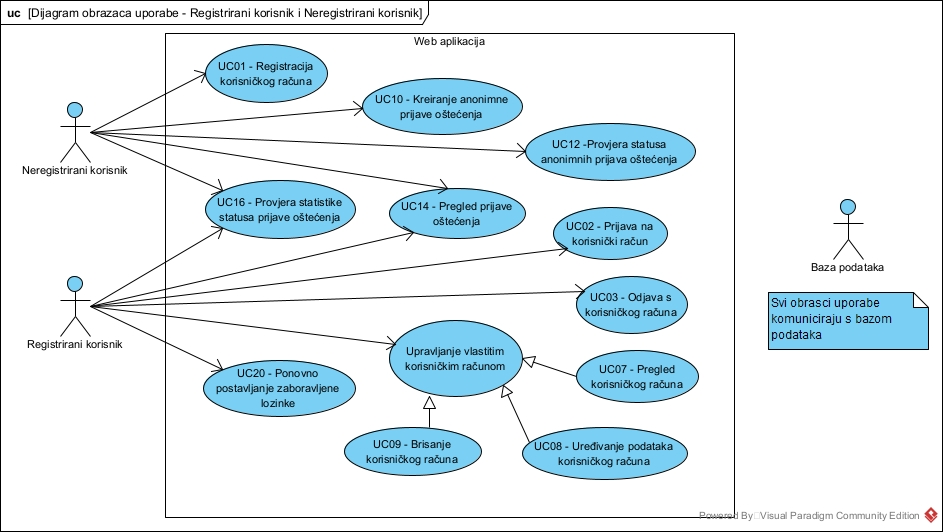
\includegraphics[scale=0.5]{slike/UC-registrirani-neregistrirani} %veličina slike u odnosu na originalnu datoteku i pozicija slike
	\centering
	\caption{Dijagram obrasca uporabe, funkcionalnost registriranog i neregistriranog korisnika}
	\label{fig:DijagramObrascaUporabeRegistriranNeregistriranKorisnik}
\end{figure}

\begin{figure}[H]
	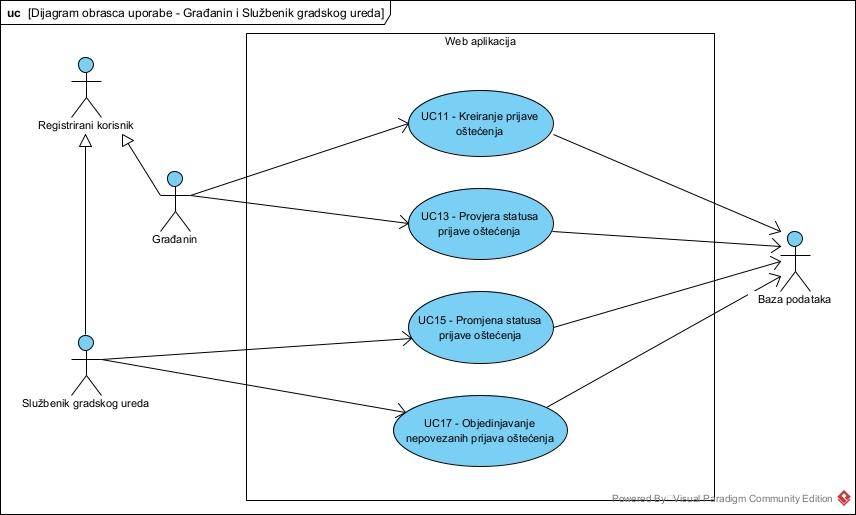
\includegraphics[scale=0.5]{slike/UC-gradanin-sluzbenik} %veličina slike u odnosu na originalnu datoteku i pozicija slike
	\centering
	\caption{Dijagram obrasca uporabe, funkcionalnost građanina i službenika gradskog ureda}
	\label{fig:DijagramObrascaUporabeGradaninSluzbenik}
\end{figure}

\begin{figure}[H]
	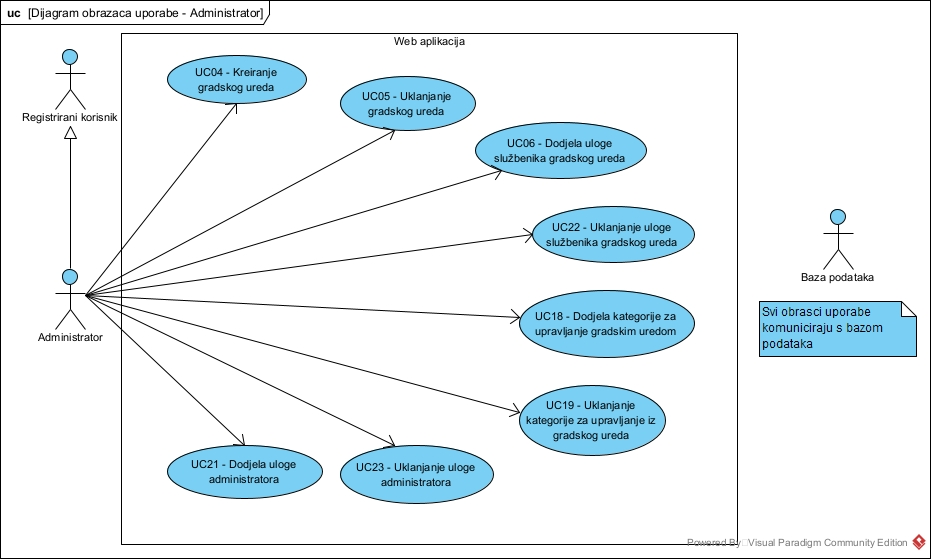
\includegraphics[scale=0.5]{slike/UC-administrator} %veličina slike u odnosu na originalnu datoteku i pozicija slike
	\centering
	\caption{Dijagram obrasca uporabe, funkcionalnost administratora}
	\label{fig:DijagramObrascaUporabeAdministrator}
\end{figure}

\eject

\subsection{Sekvencijski dijagrami}

\noindent \textbf{Obrazac uporabe UC11 - Kreiranje prijave oštećenja}

Registrirani korisnik šalje zahtjev za prikaz opcije kreiranja prijave oštećenja. Poslužitelj prikazuje stranica za kreiranje 
prijave oštećenja na kojoj korisnik unosi podatke o oštećenju. Postoje obvezni i neobvezni podaci. Dok korisnik ne unese sve 
obvezne podatke ne prikazuje se opcija za potvrdu unosa podataka. Kada unese sve obvezne podatke prikaže se opcija za potvrđivanja 
unosa podataka. Korisnik odlučuje hoće li unijeti neobvezne podatke poput fotografije oštećenja. Potvrđeni podaci spremaju se u 
bazu podataka. Ukoliko su podaci ispravni, poslužitelj prikazuje prikaz uspješnog kreiranja prijave oštećenja, a ukoliko nisu, 
poslužitelj prikazuje prikaz neuspješnog kreiranje prijave oštećenja s obrazloženjem razloga.

\begin{figure}[H]
	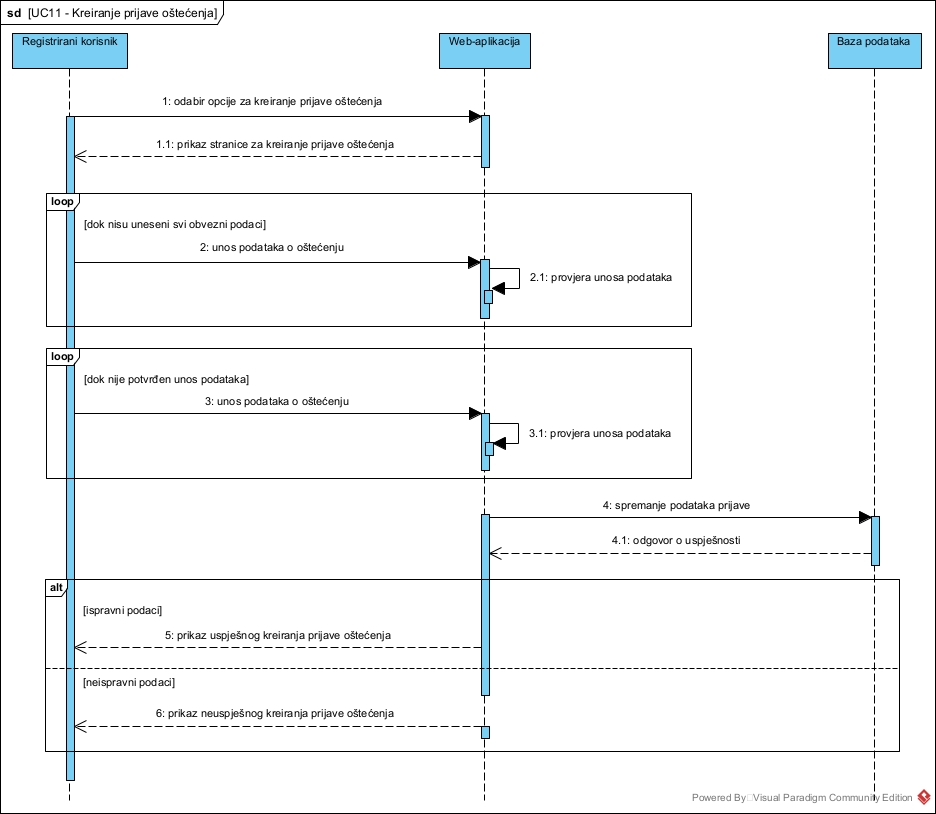
\includegraphics[scale=0.5]{slike/UC11_sekvencijski.jpg} %veličina slike u odnosu na originalnu datoteku i pozicija slike
	\centering
	\caption{Sekvencijski dijagram za UC11}
	\label{fig:SekvencijskiDijagramKreiranjePrijaveOštećenja}
\end{figure}

\noindent \textbf{Obrazac uporabe UC12 - Provjera statusa anonimne prijave oštećenja}

Neregistrirani korisnik šalje zahtjev za prikaz opcije za provjeru statusa anonimne prijave oštećenja. Poslužitelj prikazuje stranicu
za pregled statusa anonimne prijave oštećenja. Korisnik unosi jedinstveni broj prijave. Poslužitelj provjerava postoji li prijava oštećenja
s tim jedinstvenim brojem u bazi podataka. Ukoliko postoji, poslužitelj prikazuje podatke o oštećenju, a ukoliko ne postoji, poslužitelj prikazuje
poruku o neuspješnom unosu jedinstvenog broja prijave.


\begin{figure}[H]
	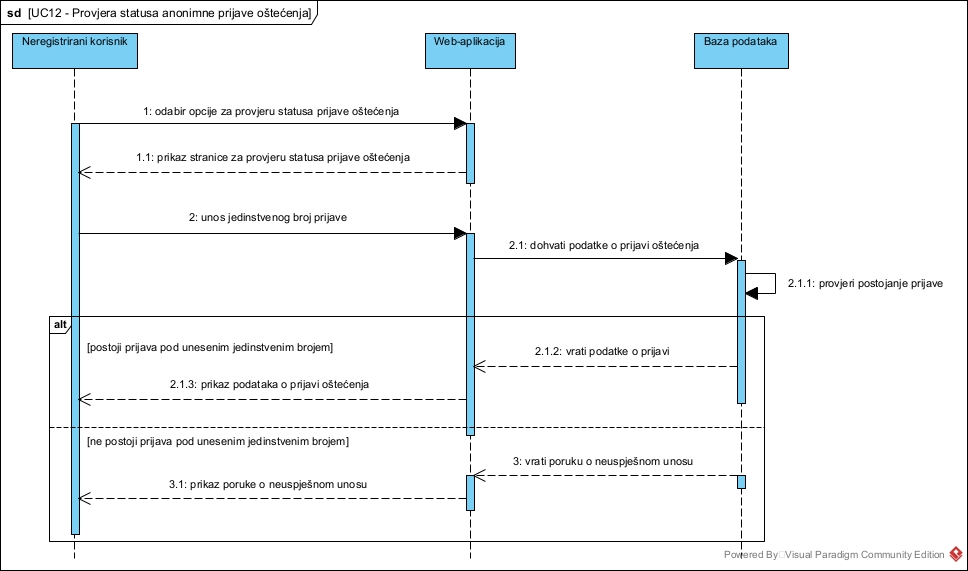
\includegraphics[scale=0.5]{slike/UC12_sekvencijski.jpg} %veličina slike u odnosu na originalnu datoteku i pozicija slike
	\centering
	\caption{Sekvencijski dijagram za UC12}
	\label{fig:SekvencijskiDijagramProvjeraStatusaAnonimnePrijaveOštećenja}
\end{figure}

\noindent \textbf{Obrazac uporabe UC15 - Promjena statusa prijave oštećenja}

Službenik gradskog ureda šalje zahtjev za prikaz popisa prijavljenih oštećenja. Poslužitelj dohvaća popis prijavljenih oštećenja iz baze 
podataka te ih prikazuje službeniku. Službenik odabire prijavu oštećenja te time šalje zahtjev za prikaz podataka o toj prijavi oštećenja. 
Poslužitelj dohvaća podatke o prijavi oštećenja te ih prikazuje službeniku. Službenik šalje zahtjev za prikaz opcije za promjenu statusa prijave
oštećenja. Poslužitelj prikazuje opciju za promjenu statusa prijave oštećenja s navedenim mogućim opcijama stanja prijave oštećenja. Službenik
odabire novi status prijave oštećenja te šalje zahtjev za promjenu statusa poslužitelju. Poslužitelj ažurira status prijave oštećenja u bazi
podataka. Poslužitelj prikazuje službeniku potvrdu o uspješnosti promjena statusa prijave oštećenja.

\begin{figure}[H]
	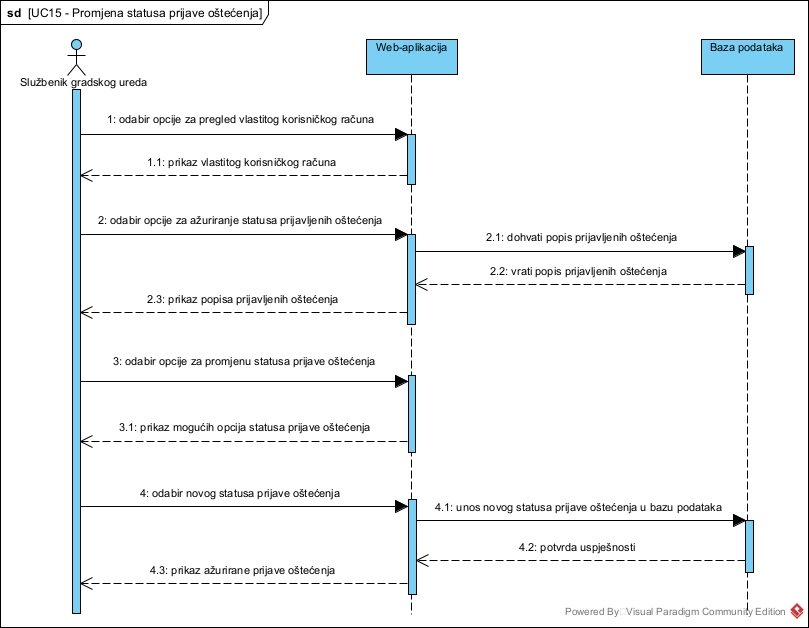
\includegraphics[scale=0.5]{slike/UC15_sekvencijski.jpg} %veličina slike u odnosu na originalnu datoteku i pozicija slike
	\centering
	\caption{Sekvencijski dijagram za UC15}
	\label{fig:SekvencijskiDijagramPromjenaStatusaPrijaveOštećenja}
\end{figure}

\noindent \textbf{Obrazac uporabe UC17 - Objedinjavanje nepovezanih prijava oštećenja}

Službenik gradskog ureda šalje zahtjev za prikaz popisa prijavljenih oštećenja. Poslužitelj dohvaća popis prijavljenih oštećenja iz baze 
podataka te ih prikazuje službeniku. Službenik odabire opciju za objedinjavanje prijava oštećenja. Poslužitelj prikazuje oznake za označavanje
prijava oštećenja. Službenik odabire prijave oštećenja. Službenik potvrđuje odabir prijava oštećenja za objedinjavanje. Poslužitelj unosi
podatke o objedinjenim prijavama oštećenja u bazu podataka. Događa se referenciranje objedinjene prijave oštećenja na postojećih prijava 
oštećenja. Po završetku, poslužitelj prikazuje službeniku gradskog ureda podatke objedinjene prijave oštećenja. 


\begin{figure}[H]
	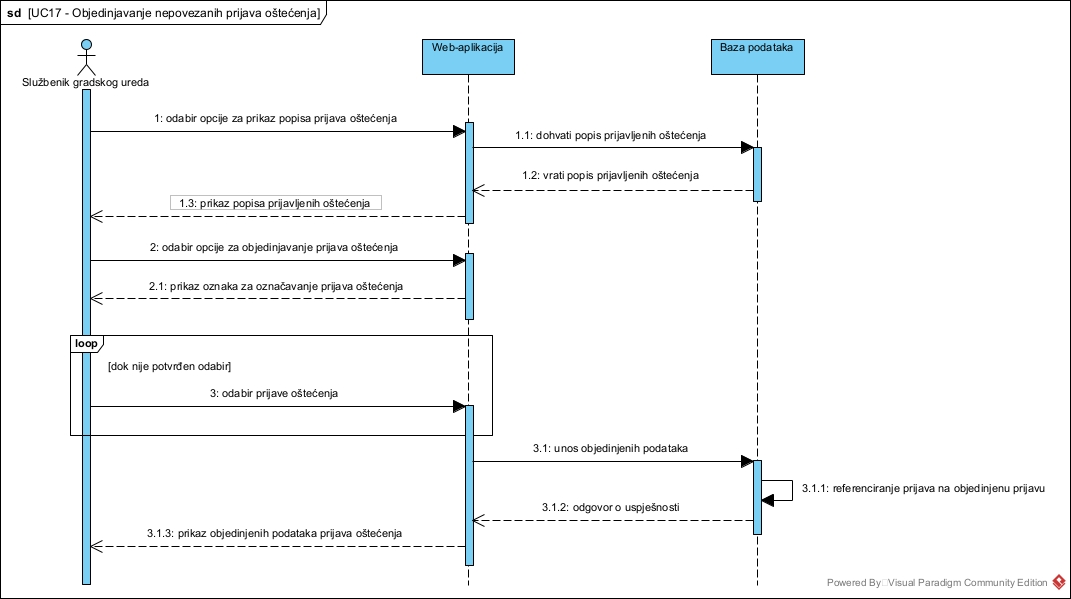
\includegraphics[scale=0.5]{slike/UC17_sekvencijski.jpg} %veličina slike u odnosu na originalnu datoteku i pozicija slike
	\centering
	\caption{Sekvencijski dijagram za UC17}
	\label{fig:SekvencijskiDijagramObjedinjavanjeNepovezanihPrijavaOštećenja}
\end{figure}

\eject

\section{Ostali zahtjevi}

\begin{packed_enum}
	\item Sustav treba podržavati rad više korisnika u stvarnom vremenu
	\item Sustav treba biti izveden kao web aplikacija
	\item Sustav treba ispravno funkcionirati na svim web preglednicima
	\item Korisničko sučelje i sustav podržavaju hrvatsku abecedu (dijakritičke znakove) pri unosu i prikazu tekstualnog sadržaja
	\item Sustav koristi hrvatski jezik i srednjoeuropsko standardno vrijeme, GMT+1
	\item Korisničko sučelje treba biti jednostavno za korištenje bez opširnih uputa
	\item Neispravno korištenje korisničkog sučelja ne smije narušiti funkcionalnost i rad sustava 
	\item Sustav ne smije omogućiti registraciju korisnika i promjenu lozinke dok nije unesena dovoljno jaka lozinka duljine od barem 8 znakove te barem jedno malo slovo, veliko slovo, znamenku i specijalni znak
	\item Sustav sprema lozinku u sigurnom obliku različitom od običnog tekstualnog formata, koristeći bcrypt hash
	\item Sustavu se pristupa s javne mreže pomoću HTTPS
	\item Pristupanje bazi podataka ne smije trajati duže od nekoliko sekundi
	\item Buduće nadogradnje sustava ne smiju narušiti postojeće funkcionalnosti sustava
\end{packed_enum}


\chapter{Arhitektura i dizajn sustava}

\noindent \\Pri analizi projektnih zahtjeva i detaljnom razmatranju uloga dionika te njihovih interakcija unutar aplikacije, odlučili smo strukturirati naš sustav na tri ključne razine: razinu klijenta, razinu web aplikacije i razinu baze podataka. Unutar ove podjele, nužno je uključiti slojeve korisničkog sučelja, aplikacijske logike i pristupa podacima. Kao model arhitekture, odabrali smo višeslojnu strukturu sličnu MVC (Model-View-Controller) stilu. MVC je oblik arhitekture softvera koji organizira aplikaciju u tri komponente:

\begin{itemize}
	\item 	\textit{Model (poslovna logika i podaci)}
	\item 	\textit{View (korisničko sučelje)}
	\item 	\textit{Controller (upravljač, posrednik između Modela i Viewa)}
\end{itemize}
\noindent Razdvajanje logike, prezentacije i upravljanja omogućuje jednostavno održavanje i razvoj aplikacije, a promjene u jednoj komponenti ne bi trebale značajno utjecati na druge. Ova arhitektura, bazirana na klijent-poslužitelj odnosu, omogućuje jasno definiranu organizaciju slojeva, a s ciljem maksimalne ponovne uporabivosti, integrirali smo i različite programske biblioteke i radne okvire. Razvojni tim je pisao kod u razvojnom okruženju IntelliJ IDEA i Visual Studio Code, a za pokretanje, konfiguraciju i puštanje u pogon, kao i neovisnost o računalu na kojem se kod izvršava, odabrali smo platforme Docker, Render i Node.JS.


\noindent \\Arhitektura web aplikacije "CestaFix" može se podijeliti na tri podsustava:
\begin{itemize}
	\item 	\textit{Web poslužitelj}
	\item   \textit{Web aplikacija}
	\item   \textit{Baza podataka}
\end{itemize}

\noindent\textbf{Web poslužitelj} je komponenta koja pruža podršku za backend sustav aplikacije i čija je ključna uloga omogućiti komunikaciju između klijenta i aplikacije. Ova interakcija odvija se putem HTTP (Hyper Text Transfer Protocol) protokola, standardnog protokola za prijenos informacija na webu. Pokretanje web aplikacije i prosljeđivanje zahtjeva aplikaciji radi daljnje obrade, inicira se upravo pomoću web poslužitelja. Za implementaciju web poslužitelja korišten je Spring Boot, Java framework, koji se ističe brzim konfiguriranjem i implementacijom web aplikacija temeljenih na Javi. Sastavljen od Model i Controller slojeva prema MVC arhitekturi, gdje se poslovna logika, kao što je upravljanje prijavama šteta, nalazi u Modelu. Web poslužitelj također omogućuje definiranje i implementaciju RESTful API-ja, što omogućuje komunikaciju između frontenda (klijenta) i backenda (poslužitelja) putem HTTP/HTTPS mrežnih protokola. Primarni zadatak Controllera unutar web poslužitelja je obrađivanje HTTP zahtjeva koji pristižu iz frontend dijela aplikacije, izvršavanje odgovarajuće funkcionalnosti te slanje odgovora. Dodatno, Spring Boot omogućuje učinkovito upravljanje stanjem aplikacije, uključujući praćenje stanja sesija za registrirane korisnike.
\newline
\textbf{\\Web preglednik} je softver koji djeluje kao posrednik između poslužitelja i klijenta, omogućujući korisniku prikaz web sadržaja. Osnovna funkcionalnost web preglednika ostvarena je pri slanju HTTP zahtjeva poslužitelju te prijemu i interpretaciji HTTP odgovora. Web preglednici djeluju kao prevoditelji, omogućavajući korisnicima vizualizaciju web sadržaja kroz sučelje preglednika, dekodiranjem informacija dobivenih iz HTTP odgovora.
\newline
\textbf{\\Web aplikacija} Web aplikacija je kompleksni softverski sustav koji se sastoji od frontend i backend dijelova:
\begin{itemize}
	\item \textbf{Frontend} (Klijent) predstavlja korisničko sučelje putem kojeg korisnici ostvaruju interakciju sa sustavom. Ostvaren je korištenjem JavaScript programskog jezika, za potrebu upravljanja događajima na korisničkom sučelju, i React radnog okvira, što omogućuje kreiranje dinamičnog i intuitivnog korisničkog sučelja, čime se ostvaruje ugodno korisničko iskustvo. Frontend je strukturiran u komponente, što olakšava održavanje i ponovnu uporabu koda. Komunicira s backendom kroz HTTPS zahtjeve te pritom omogućuje prijenos podataka i ažuriranje informacija o prijavama šteta. Kroz klijentsku logiku, frontend provodi validaciju unesenih podataka kako bi osigurao ispravnost prije slanja na backend. Responsivni dizajn osigurava konzistentno korisničko iskustvo na različitim uređajima.
	\item \textbf{Backend} (Poslužitelj) je dio sustava unutar kojeg se obrađuju zahtjevi i izvršavaju daljnje radnje. Kako bi se postiglo "razdvajanje zabrinutosti", organiziran je na kontrolere, servise i repozitorije. Controlleri imaju ključnu ulogu u obradi ulaznih zahtjeva (HTTP zahtjeva) omogučujući organizaciju i upravljanje tijekom rukovanja zahtjevima u backend dijelu aplikacije kao i pozivanje odgovarajućih metoda u Modelu te slanje odgovora klijentskom dijelu. Servisi u backendu na učinkovit i organiziran način obavljaju poslovnu logiku i specifične funkcionalnosti koje su potrebne za obradu zahtjeva, koji dolaze s frontend dijela aplikacije. Repozitoriji imaju ključnu ulogu u komunikaciji s bazom podataka, odnosno omogućuju servisima da abstrahiraju detalje interakcije s bazom podataka, pružajući im jednostavan i konzistentan način komunikacije s podacima. Backend je ostvaren korištenjem Java programskog jezika i Spring Boot radnog okvira. Također, pruža RESTful API-je koji omogućuju komunikaciju između klijenta i servera te definiraju kako resursi (poput prijava šteta) mogu biti stvoreni, ažurirani i dohvaćeni. Osim toga backend sadrži i DTO-e (Data Transfer Objects) za prijenos podataka između različitih dijelova sustava odnosno slojeva aplikacije.
\end{itemize}

\noindent \textbf{Baza podataka} je podatkovni sloj koji se koristi za sigurnu pohranu podataka te je detaljnije opisana u sljedećem poglavlju.

\begin{figure}[H]
	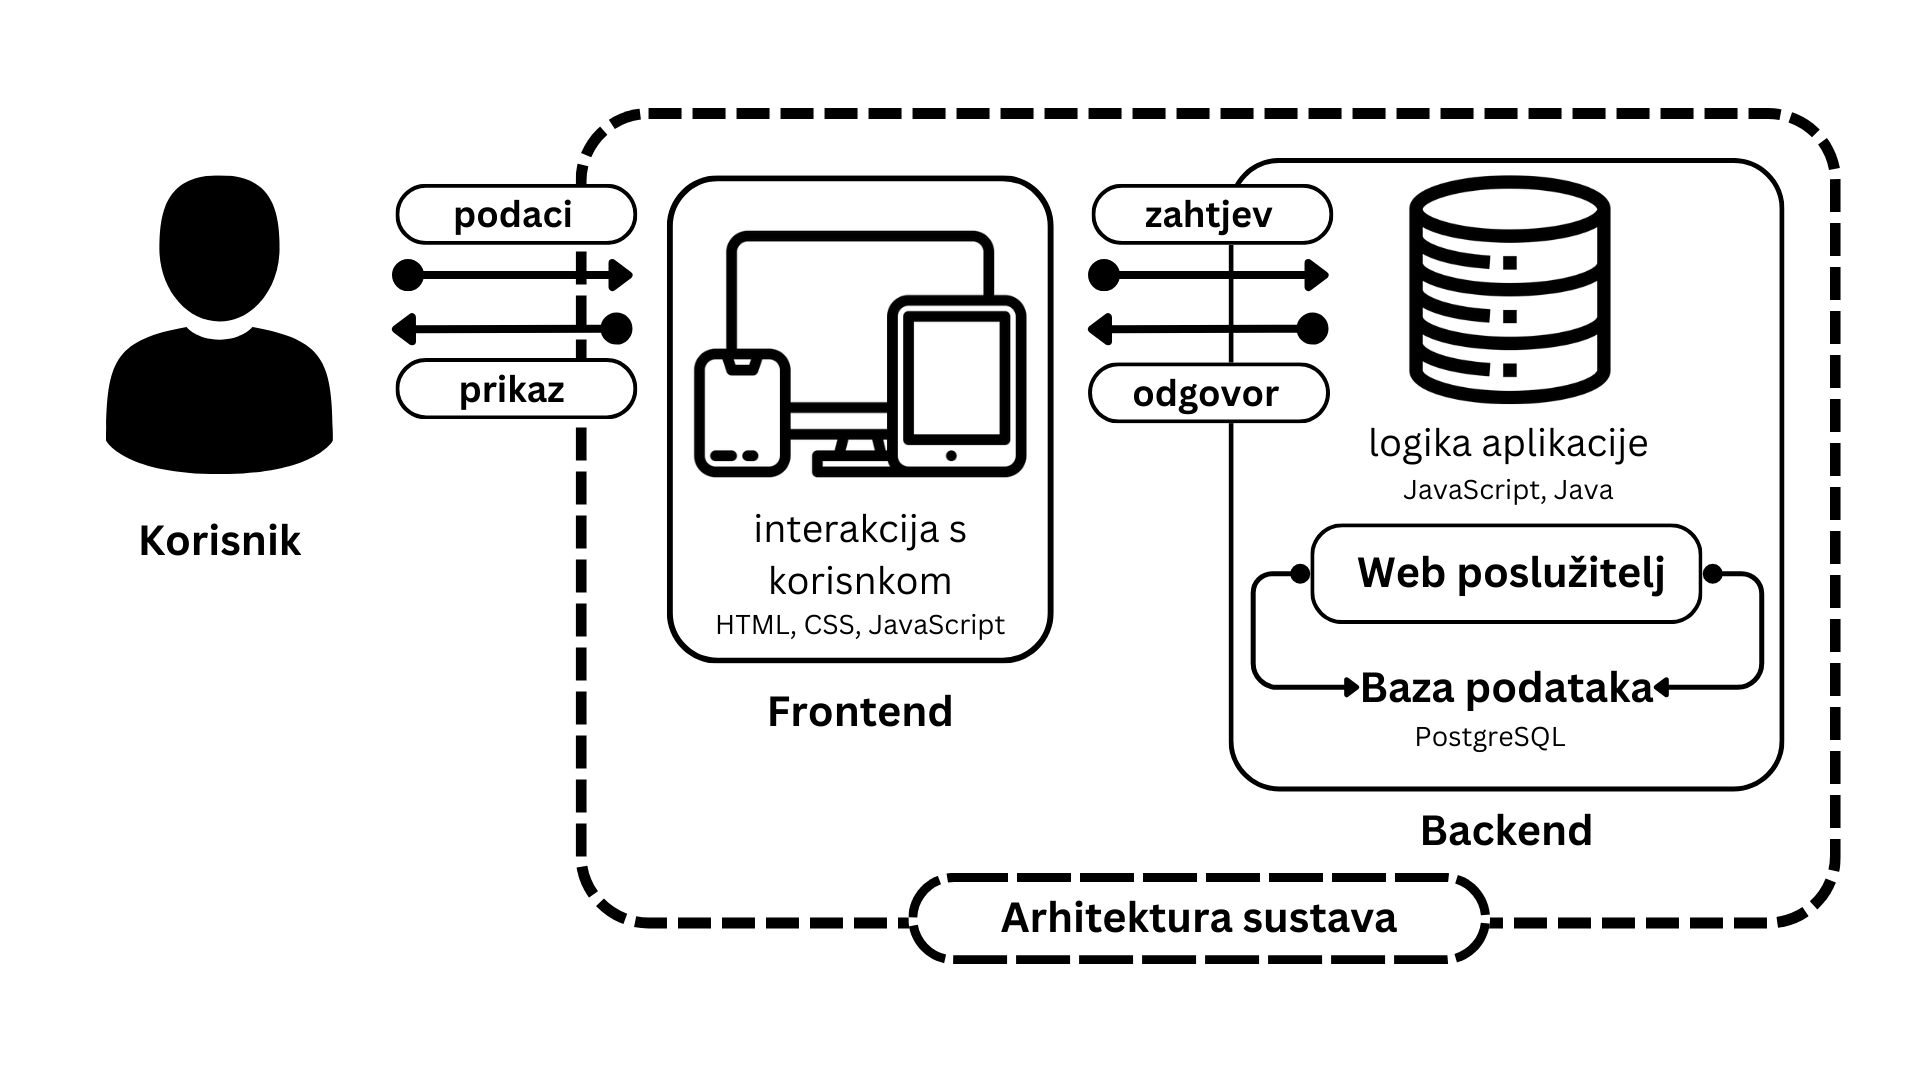
\includegraphics[scale=0.25]{slike/Arhitektura_sustava.png} %veličina slike u odnosu na originalnu datoteku i pozicija slike
	\centering
	\caption{Arhitektura sustava}
	\label{fig:Arhitektura}
\end{figure}


\section{Baza podataka}

\noindent Sustav je temeljen na uporabi relacijske baze podataka implementirane u PostgreSQL-u gdje su entiteti modelirani kao tablice koje posjeduju svoje jedinstveno ime i skup atributa.
Odabir relacijske baze podataka proizlazi iz potrebe za lakšim ostvarenjem naših potreba za upravljanjem podacima pri prijavljivanju oštećenja i njihovoj sanaciji
odnosno kako bismo što jednostavnije modelirali sustav prema stvarnom svijetu.
Ova baza podataka ključna je za sigurnost podataka i brz pristup, pohranu, umetanje, izmjenu te dohvat podataka koje sustav koristi za daljnju obradu.
Baza podataka ove aplikacija sadrži sljedeće entitete:
\begin{packed_item}
	\item \textit{Users}
	\item \textit{Reports}
	\item \textit{CityDept}
	\item \textit{Category}
	\item \textit{Problems}
	\item \textit{Photo}
\end{packed_item}



\subsection{Opis tablica}

\noindent \textbf{Users} je entitet koji sadrži sve bitne informacije o korisnicima i njihovim ulogama unutar aplikacije.
Sastoji se od atributa: user\_id, firstname, lastname, email, password, role i city\_dept\_id.
Povezan je vezom \textit{Many-to-One} s entitetom CityDept preko atributa city\_dept\_id i vezom \textit{One-to-Many} s entitetom Reports preko atributa user\_id.


\begin{longtblr}[
	label=none,
	entry=none
	]{
	width = \textwidth,
	colspec={|X[6,l]|X[6, l]|X[20, l]|},
	rowhead = 1,
	} %definicija širine tablice, širine stupaca, poravnanje i broja redaka naslova tablice
	\hline \SetCell[c=3]{c}{\textbf{Users}}                                                                           \\ \hline[3pt]
	\SetCell{LightGreen}user\_id       & INT     & jedinstveni identifikator korisnika                                \\ \hline
	firstname                          & VARCHAR & ime korisnika                                                      \\ \hline
	lastname                           & VARCHAR & prezime korisnika                                                  \\ \hline
	email                              & VARCHAR & e-mail adresa korisnika                                            \\ \hline
	password                           & VARCHAR & hash lozinke korisnika                                             \\ \hline
	role                               & VARCHAR & uloga korisnika                                                    \\ \hline
	\SetCell{LightBlue} city\_dept\_id & INT     & jedinstveni identifikator gradskog ureda (citydept.city\_dept\_id) \\ \hline
\end{longtblr}


\noindent\textbf{Reports} je entitet koji sadrži sve bitne informacije o prijavama oštećenja.
Sastoji se od atributa: report\_id, user\_id, title, description, address, report\_time, status, problem\_id, longitude, latitude i business\_id.
Povezan je vezom \textit{Many-to-One} s entitetom Problems preko atributa problem\_id, vezom \textit{Many-to-One} s entitetom Users preko atributa user\_id i vezom \textit{One-to-Many} s entitetom Photo preko atributa report\_id.
\begin{longtblr}[
	label=none,
	entry=none
	]{
	width = \textwidth,
	colspec={|X[6,l]|X[6, l]|X[20, l]|},
	rowhead = 1,
	} %definicija širine tablice, širine stupaca, poravnanje i broja redaka naslova tablice
	\hline \SetCell[c=3]{c}{\textbf{Reports}}                                                                \\ \hline[3pt]
	\SetCell{LightGreen}report\_id  & INT       & jedinstveni identifikator prijave                          \\ \hline
	\SetCell{LightBlue} user\_id    & INT       & jedinstveni identifikator korisnika (users.user\_id)       \\ \hline
	title                           & VARCHAR   & naziv prijave/oštećenja                                    \\ \hline
	description                     & TEXT      & opis oštećenja                                             \\ \hline
	address                         & VARCHAR   & adresa oštećenja                                           \\ \hline
	report\_time                    & TIMESTAMP & vrijeme podnošenja prijave                                 \\ \hline
	status                          & VARCHAR   & status prijave                                             \\ \hline
	longitude                       & DOUBLE    & geografska dužina lokacije oštećenja                       \\ \hline
	latitude                        & DOUBLE    & geografska širina lokacije oštećenja                       \\ \hline
	business\_id                    & UUID      & jedinstveni identifikator anonimne prijave                 \\ \hline
	\SetCell{LightBlue} problem\_id & INT       & jedinstveni identifikator oštećenja (problems.problem\_id) \\ \hline
\end{longtblr}

\noindent\textbf{CityDept} je entitet koji sadrži sve bitne informacije o gradskim uredima.
Sastoji se od atributa: city\_dept\_id, city\_dept\_name i category\_id.
Povezan je vezom \textit{One-to-Many} s entitetom Users preko atributa city\_dept\_id i vezom \textit{One-to-One} s entitetom Category preko atributa category\_id.
\begin{longtblr}[
	label=none,
	entry=none
	]{
	width = \textwidth,
	colspec={|X[6,l]|X[6, l]|X[20, l]|},
	rowhead = 1,
	} %definicija širine tablice, širine stupaca, poravnanje i broja redaka naslova tablice
	\hline \SetCell[c=3]{c}{\textbf{CityDept}}                                                                            \\ \hline[3pt]
	\SetCell{LightGreen}city\_dept\_id & INT     & jedinstveni identifikator gradskog ureda                               \\ \hline
	city\_dept\_name                   & VARCHAR & naziv gradskog ureda                                                   \\ \hline
	\SetCell{LightBlue} category\_id   & INT     & jedinstveni identifikator kategorije oštećenja (category.category\_id) \\ \hline
\end{longtblr}

\noindent\textbf{Category} je entitet koji sadrži sve bitne informacije o kategoriji oštećenja.
Sastoji se od atributa: category\_id i category\_name.
Povezan je vezom \textit{One-to-Many} s entitetom Problems preko atributa category\_id i vezom \textit{One-to-One} s entitetom CityDept preko atributa category\_id.
\begin{longtblr}[
	label=none,
	entry=none
	]{
	width = \textwidth,
	colspec={|X[6,l]|X[6, l]|X[20, l]|},
	rowhead = 1,
	} %definicija širine tablice, širine stupaca, poravnanje i broja redaka naslova tablice
	\hline \SetCell[c=3]{c}{\textbf{Category}}                                                  \\ \hline[3pt]
	\SetCell{LightGreen}category\_id & INT     & jedinstveni identifikator kategorije oštećenja \\ \hline
	category\_name                   & VARCHAR & naziv kategorije oštećenja                     \\ \hline
\end{longtblr}

\noindent\textbf{Problems} je entitet koji sadrži sve bitne informacije o prijavljenom oštećenju.
Sastoji se od atributa: problem\_id, longitude, latitude, status i category\_id.
Povezan je vezom \textit{One-to-Many} s entitetom Reports preko atributa problem\_id i vezom \textit{Many-to-One} s entitetom Category preko atributa category\_id.
\begin{longtblr}[
	label=none,
	entry=none
	]{
	width = \textwidth,
	colspec={|X[6,l]|X[6, l]|X[20, l]|},
	rowhead = 1,
	} %definicija širine tablice, širine stupaca, poravnanje i broja redaka naslova tablice
	\hline \SetCell[c=3]{c}{\textbf{Problems}}                                                                           \\ \hline[3pt]
	\SetCell{LightGreen}problem\_id  & INT     & jedinstveni identifikator oštećenja                                     \\ \hline
	longitude                        & DOUBLE  & geografska dužina lokacije oštećenja                                    \\ \hline
	latitude                         & DOUBLE  & geografska širina lokacije oštećenja                                    \\ \hline
	status                           & VARCHAR & status oštećenja                                                        \\ \hline
	\SetCell{LightBlue} category\_id & INT     & jedinstveni identifikator kategorije oštećenja  (category.category\_id) \\ \hline
\end{longtblr}


\noindent\textbf{Photo} je entitet koji sadrži sve bitne informacije vezane za sliku oštećenja.
Sastoji se od atributa: photo\_id, photo\_data i report\_id.
Povezan je vezom \textit{Many-to-One} s entitetom Reports preko atributa report\_id.

\begin{longtblr}[
	label=none,
	entry=none
	]{
	width = \textwidth,
	colspec={|X[6,l]|X[6, l]|X[20, l]|},
	rowhead = 1,
	} %definicija širine tablice, širine stupaca, poravnanje i broja redaka naslova tablice
	\hline \SetCell[c=3]{c}{\textbf{Photo}}                                                       \\ \hline[3pt]
	\SetCell{LightGreen}photo\_id & INT   & jedinstveni identifikator slike (photo.photo\_id)     \\ \hline
	photo\_data                   & BYTEA & slika oštećenja                                       \\ \hline
	\SetCell{LightBlue}report\_id & INT   & jedinstveni identifikator prijave (report.report\_id) \\ \hline
\end{longtblr}


\subsection{Dijagram baze podataka}

\begin{figure}[H]
	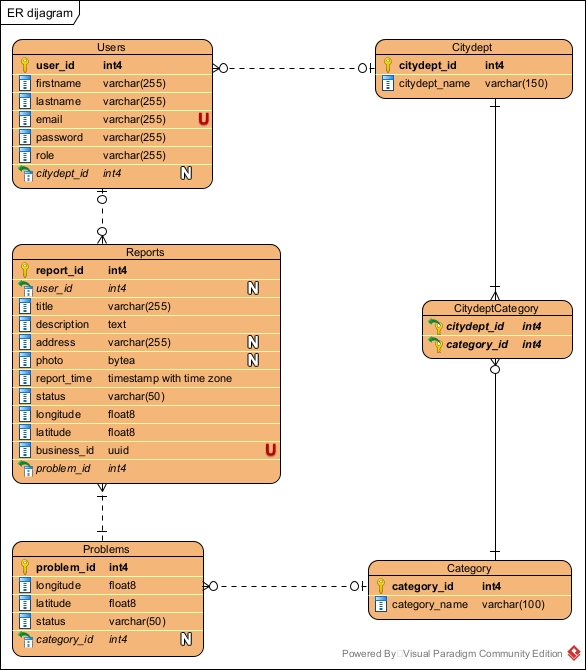
\includegraphics[scale=0.75]{slike/ERD-model} %veličina slike u odnosu na originalnu datoteku i pozicija slike
	\centering
	\caption{E-R dijagram baze podataka}
	\label{fig:ERdijagramBazePodataka}
\end{figure}

\eject


\section{Dijagram razreda}

Na slikama 4.3, 4.4, 4.5 i 4.6 prikazani su razredi koji pripadaju \textit{backend} dijelu
s arhitekturom podijeljenom na kontrolere, repozitorije i servise te uključuje DTO
(Data Transfer Object) i modele. \newline

Na slikama 4.3 i 4.4 prikazani su razredi koji nasljeđuju Controller razred. Metode implementirane u tim razredima
upravljaju i rukuju DTO-ima koji su dohvaćeni pomoću metoda implementiranih u Model razredima. Omogućuju
logiku interakcije i promjene. Kontroler AuthenticationController omogućuje registraciju i prijavu korisnika.
Kontroler ReportController omogućuje interakcije s prijavom oštećenja, dok kontroler ProblemController omogućuje
interakcije s objedinjenim problemima oštećenja s istom temom i lokacijom. Kontroler UserController omogućuje
interakcije i promjene povezane s registriranim korisnicima. Kontroler CityDeptController omogućuje
interakcije i promjene povezane s gradskim uredima. Kontroler PhotoController omogućuje interakciju i promjene
vezane za slike oštećenja. Kontroler CategoryController omogućuje interakciju i promjene vezane za
kategorije oštećenja. Kontroler ExceptionController omogućuje interakcije vezane za iznimke.

\begin{figure}[H]
	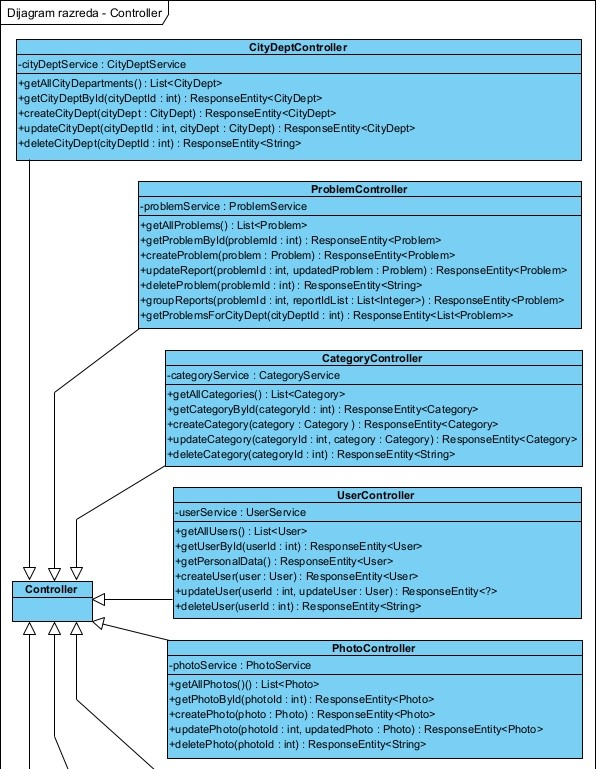
\includegraphics[scale=1.0]{slike/DR-controller1} %veličina slike u odnosu na originalnu datoteku i pozicija slike
	\centering
	\caption{Dijagram razreda - dio Controllers - prvi dio}
	\label{fig:DijagramRazredaControllers}
\end{figure}

\begin{figure}[H]
	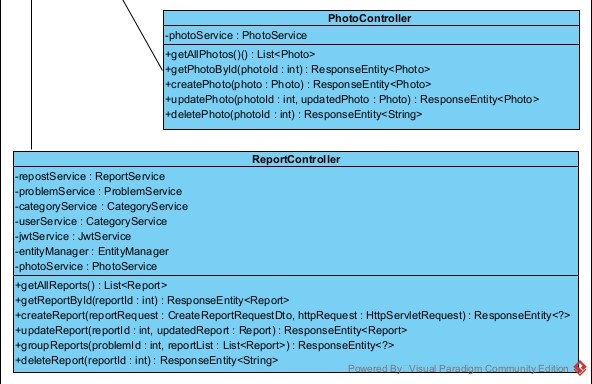
\includegraphics[scale=1.0]{slike/DR-controller2} %veličina slike u odnosu na originalnu datoteku i pozicija slike
	\centering
	\caption{Dijagram razreda - dio Controllers - drugi dio}
	\label{fig:DijagramRazredaControllers}
\end{figure}

Na slici 4.4 prikazani su razredi koji pripadaju DTO. Data Transfer Objects (DTO) omogućavaju
razmjenu podataka između procesa i slojeva. RegisterRequestDto služi za registraciju korisnika.
LoginRequestDto služi za prijavu korisnika. AuthenticationResponseDto sastoji se od jwt tokena koji se vraća
kada se korisnik registrira ili ulogira. ReportRequestDto služi za kreiranje podataka o prijavi
oštećenja i problema.

\begin{figure}[H]
	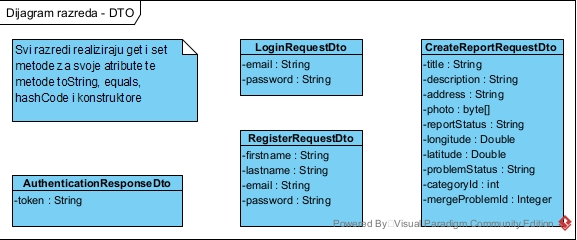
\includegraphics[scale=0.60]{slike/DR-DTO.jpg} %veličina slike u odnosu na originalnu datoteku i pozicija slike
	\centering
	\caption{Dijagram razreda - dio DTO}
	\label{fig:DijagramRazredaDTO}
\end{figure}

Na slici 4.5 prikazi su razredi koji pripadaju Model razredima. Oni preslikavaju strukturu baze podataka
u aplikaciji. Komuniciraju s bazom podataka te vraćaju podatke iz nje. Razred User predstavlja registriranog
korisnika koji je unio nužne podatke u sustav. Razred Report predstavlja prijavu oštećenja za koju je korisnik
unio potrebne i opcionalne podatke. Razred Problem predstavlja prijavu problema koja predstavlja jednu ili više
prijava oštećenja objedinjene u prijavu problema sa zajedničkom temom i lokacijom. Razred Category predstavlja
kategoriju oštećenja koju korisnik može odabrati za prijavljeno oštećenje, odnosno koju gradski ured može dobiti
na upravljanje oštećenjima. Razred CityDept predstavlja gradski ured koji upravlja jednom kategorijom oštećenja
koju im je administrator dodijelio. Enumeracija Role predstavlja ulogu koju registrirani korisnik ima. Razred
Photo predstavlja fotografiju oštećenja koju je korisnik dodao prilikom prijave oštećenja.

\begin{figure}[H]
	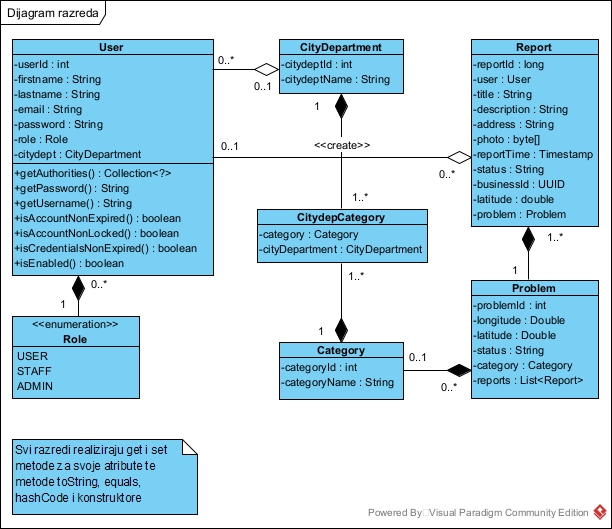
\includegraphics[scale=0.60]{slike/DR-model.jpg} %veličina slike u odnosu na originalnu datoteku i pozicija slike
	\centering
	\caption{Dijagram razreda - dio Model}
	\label{fig:DijagramRazredaModel}
\end{figure}

\eject

\section{Dijagram stanja}

Dijagram stanja, poznat i kao state machine diagram, je ponašajni UML-dijagram koji se koristi za jasno definiranje mogućih stanja objekta, identifikaciju prijelaza između tih stanja i prikaz ponašanja sustava u različitim situacijama.
Na slici 4.7 prikazan je dijagram stanja za prijavljenog korisnika. Nakon prijave, korisniku se prikazuje početna stranica s kartografskim prikazom na kojem su crvenim markerima označene već podnesene prijave određenih šteta na javnim površinama.
Odabirom nekog crvenog markera, korisniku se prikazuju informacije o konkretnoj podnesenoj prijavi. Sličnu funkcionalnost korisnik ostvaruje upisom identifikacijskog broja prijave u zaglavlju čime mu se prikazuju informacije, odnosno status neke od vlastitih podnesenih prijava. Osim pregleda statusa podnesenih šteta, pomoću zaglavlja aplikacije korisnik može pristupiti svom korisničkom računu, pregledati statistiku svih do tog trenutka podnesenih prijava te pristupiti podnošenju nove prijave. Prilikom podnošenja nove prijave, osim unošenja podataka o nastaloj šteti, korisnik može odabrati sliku s vlastitog uređaja i odabrati lokaciju štete na karti. Također, pomoću padajućeg izbornika u zaglavlju, korisnik se može odjaviti iz sustava. S obzirom na to da je zaglavlje zastupljeno na svim stranicama aplikacije, korisnik svim navedenim opcijama vezanim uz zaglavlje može pristupiti neovisno o tome gdje se nalazi unutar aplikacije. Pristupom u vlastiti korisnički račun, omogućen je pregled i uređivanje osobnih podataka, pregled podnesenih prijava korisnika kao i brisanje računa. Ako korisnik prilikom pregleda informacija vlastitih podnesenih prijava, odabere jednu od njih, pristupa informacijama o svim bliskim prijavama odabrane prijave.
\begin{figure}[H]
	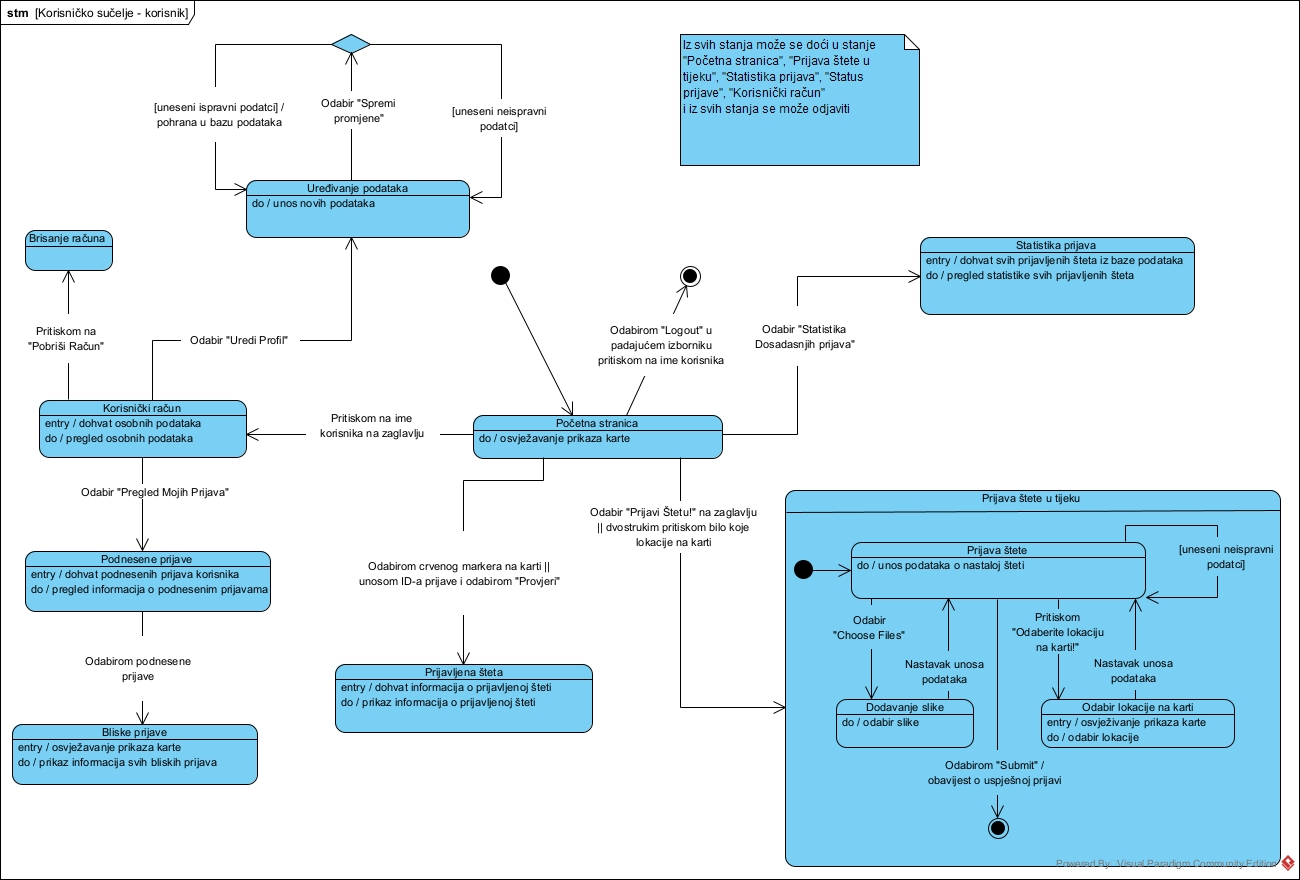
\includegraphics[scale=0.35]{slike/DS.jpg} %veličina slike u odnosu na originalnu datoteku i pozicija slike
	\centering
	\caption{Dijagram stanja}
	\label{fig:DijagramStanja}
\end{figure}

\eject

\section{Dijagram aktivnosti}

UML-dijagrami aktivnosti (activity diagrams) predstavljaju ponašajne dijagrame koji se koriste za modeliranje i grafički prikaz dinamičkog ponašanja sustava.
Ovi dijagrami vizualiziraju izvođenje aktivnosti kroz niz akcija koje kontroliraju tokove i objekte, s posebnim naglaskom na slijed i uvjete toka.
Dijagrami aktivnosti omogućuju jasno predstavljanje redoslijeda izvođenja aktivnosti, čime olakšavaju razumijevanje dinamike sustava.
Na dijagramu aktivnosti sa slike 4.8 prikazan je proces podnošenja nove prijave štete neprijavljenog korisnika.
Korisnik se prijavi u sustav, zatim odabirom lokacije na karti ili odabirom "Prijavi Štetu!" na zaglavlju, unosi podatke o nastaloj šteti u prikazanoj formi za prijavu.
Ako su podaci neispravno uneseni, korisniku se omogućuje ponovni upis podataka, a ako su podaci ispravni, spremaju se u bazu podataka te se korisniku prikazuje potvrda o uspješno podnesenoj prijavi zajedno s identifikacijskim brojem prijave, kako bi mogao provjeriti status podnesene prijave. Korisnik je pri završetku procesa pozicioniran ponovno na početnu stranicu.

\begin{figure}[H]
	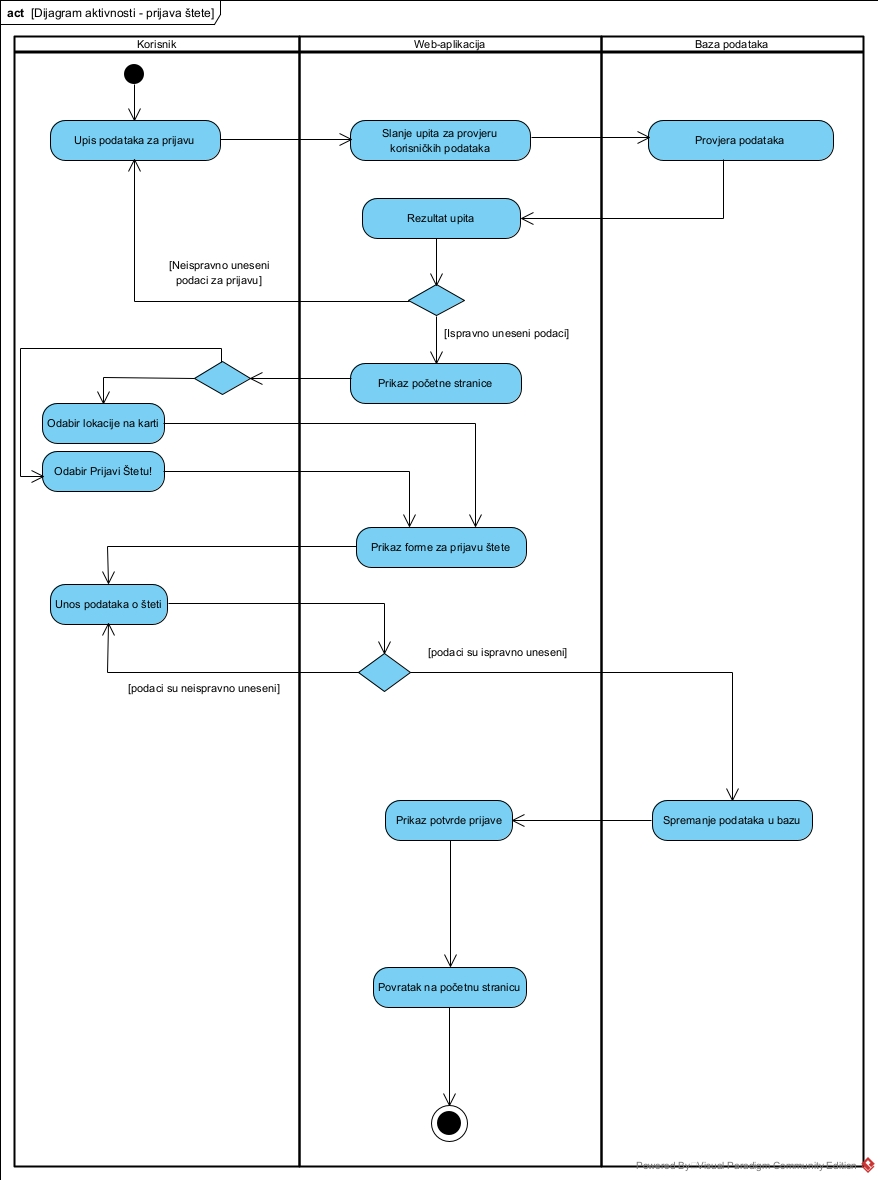
\includegraphics[scale=0.5]{slike/DA.jpg} %veličina slike u odnosu na originalnu datoteku i pozicija slike
	\centering
	\caption{Dijagram aktivnosti}
	\label{fig:DijagramAktivnosti}
\end{figure}

\eject
\section{Dijagram komponenti}

Dijagram komponenti prikazan je na slici 4.9 te služi za vizualizaciju organizacije i međuovisnosti implementacijskih
komponenata (interna struktura) te odnos programske potpore prema okolini. Sustavu se pristupa preko web preglednika pomoću sučelja HTTP\_REQUEST
na kojem se poslužuju datoteke koje pripadaju \textit{frontend} dijelu aplikacije. \textit{Frontend} dio nazvan React Frontend
sastoji se od komponenti React View, React router, ReactJS, Index.js, Content.js, React leaflet te sučelja REST\_API i MAP\_API.
React View komponenta komunicira s \textit{backendom} preko sučelja REST\_API i razmjenjuje podatke s \textit{backendom} u
JSON formatu, te ovisno o korisnikovim akcijama osvježava prikaz na stranici. Komponenta React router na temelju URL-a
odlučuje koja će se stranica prikazati, odnosno datoteka dohvatiti. Komponenta ReactJS je centralna biblioteka za React
preko koje se dobivaju gotove komponente za prikaz. Komponenta Index.js služi kao početna komponenta unutar koje se nalazi
organizirana hijerarhija ostalih elemenata za prikaz. Jedan od njih je komponenta Content.js koja služi za ostvarivanje
prikaza karte. Integraciju interaktivnih karata i manipulaciju geografskih podataka s React aplikacijama omogućava biblioteka
React leaflet prikazana komponentom React leaflet. Sučelje MAP\_API koristi se za razmjenu podataka s vanjskom komponentom
Openstreetmaps. \textit{Backend} dio nazvan Spring Boot backend sastoji se od komponenti RestController, JPA repository,
Controller, Service, Model, Repository, DTO te sučelja REST\_API, PSQL, JPA i GEOCODING\_API. Komponenta RestController komunicira
s \textit{frontendom} preko sučelja REST\_API i razmjenjuje podatke u JSON formatu. Komponenta JPA repository predstavlja
dio Spring Data JPA koji omogućava jednostavan pristup podacima u bazi podataka koristeći PSQL sučelje za komuniciranje i
razmjenu podataka s vanjskom komponentnom PostgreSQL baza podataka te sučelja JPA za komunikaciju s komponentnom Repository.
Komponenta Controller prima zahtjeve, provjerava ih te šalje odgovore na dobivene zahtjeve prema klijentskoj strani. Komponenta
Service prima zahtjeve od Controller, obrađuje ih i prosljeđuje komponentni Repository. Komponenta Model predstavlja entitete
koji se pohranjuju u bazi podataka. Komponenta DTO predstavlja oblik objekta koji se koristi za prijenos podataka između
dijelova aplikacije. Sučelje GEOCODING\_API komunicira s vanjskom komponentom Geocoding koja služi za pretvaranje adrese
u geografske koordinate i obrnuto.


\begin{figure}[H]
	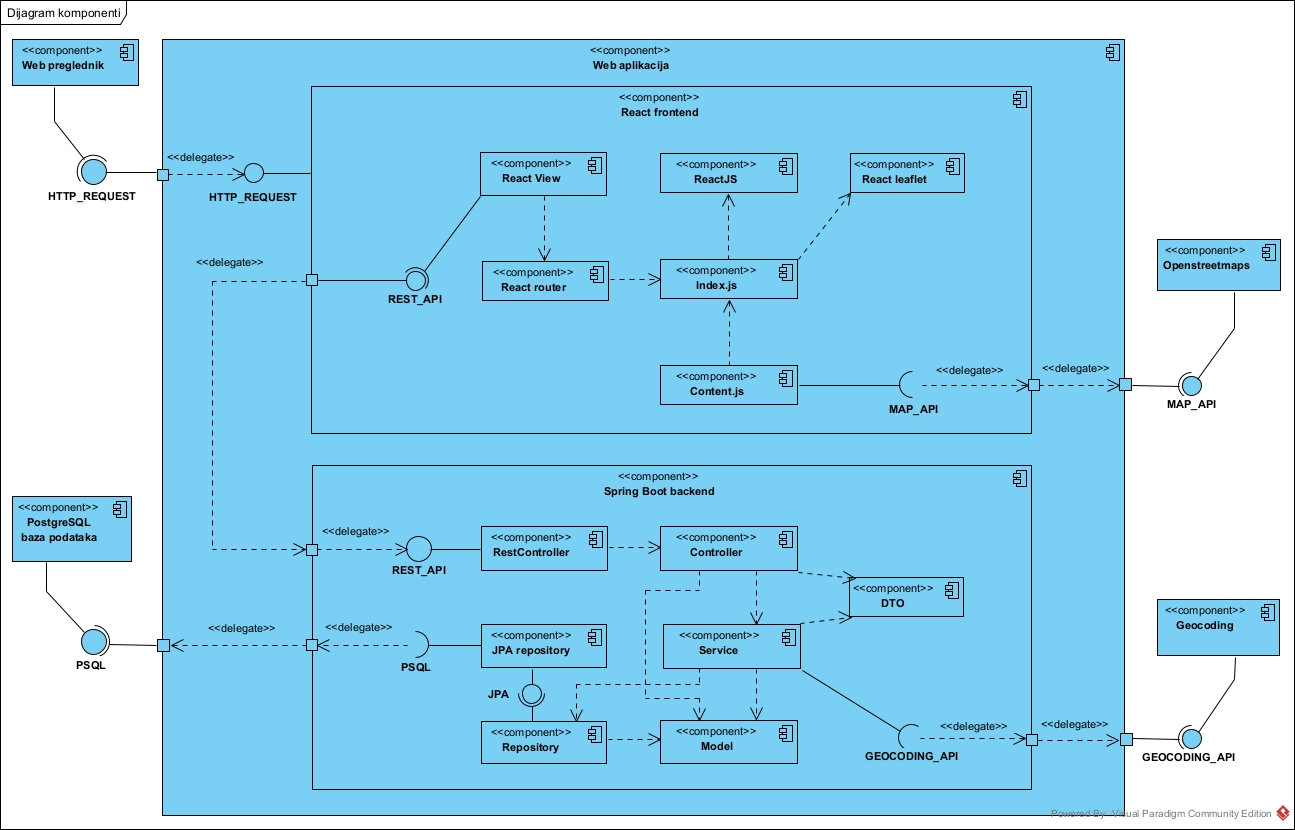
\includegraphics[scale=0.35]{slike/DK.jpg} %veličina slike u odnosu na originalnu datoteku i pozicija slike
	\centering
	\caption{Dijagram komponenti}
	\label{fig:DijagramKomponenti}
\end{figure}
\chapter{Implementacija i korisničko sučelje}
		
		
		\section{Korištene tehnologije i alati}
		
			 Komunikacija u timu realizirana je korištenjem aplikacije \textbf{\href{https://discord.com/}{Discord}}. 
			 Discord je društvena platforma na kojoj korisnici imaju mogućnost komuniciranja tekstualnim porukama, glasovnim
			 pozivima, videopozivima, medijima i datotekama u privatnim porukama ili kao dio zajednice koju nazivaju server. 
			 Za izradu UML dijagrama korišten je alat \textbf{\href{https://www.visual-paradigm.com/}{Visual Paradigm}}. Visual 
			 Paradigm je grafički alat koji omogućava jednostavno modeliranje mnogo različitih tipova UML dijagrama, poput 
			 dijagrama obrazaca uporabe, sekvencijskih dijagrama, dijagrama razreda, dijagrama stanja, dijagrama aktivnosti, 
			 dijagrama komponenata, ERD modela baze podataka i mnogih drugih. Za upravljanje izvornim kodom korišten je 
			 \textbf{\href{https://git-scm.com/}{Git}}. Git je open-source distribuirani sustav za upravljanje različitim 
			 verzijama datoteka. Udaljeni repozitorij projekta je dostupan na web platformi \textbf{\href{https://github.com/}{GitHub}}.
			 GitHub pruža usluge spremanja i upravljanja kodom. Koristi se Git-om kako bi omogućio upravljanje različitim 
			 verzijama datoteka. Također, GitHub omogućava dokumentiranje programske podrške pomoću wiki-ja.

			 Kao razvojno okruženje korišteni su \textbf{\href{https://code.visualstudio.com/}{Visual Studio Code}} 
			 i \textbf{\href{https://www.jetbrains.com/idea//}{Intellij IDEA}}. Visual Studio Code je uređivač teksta
			 razvijen u tvrtki Microsoft. Prvenstveno se koristi za razvoj računalnih sustava na operacijskom sustavu Windows. 
			 Korišten je za razvoj programske podrške na \textit{frontendu} i razvoj dokumentacije. Intellij IDEA je integrirano razvojno 
			 okruženje (IDE) razvijeno u tvrtki JetBrains. Usmjereno je na razvoj Java aplikacija, no podržava niz drugih jezika i 
			 tehnologija. Korišten je za razvoj programske podrške na \textit{backendu}.

			 Aplikacija je napisana koristeći radni okvir \textbf{\href{https://spring.io/projects/spring-boot}{Spring Boot}} i jezik 
			 \textbf{\href{https://www.java.com/en/}{Java}} za izradu \textit{backenda} te jezik \textbf{\href{https://www.javascript.com/}{JavaScript}} 
			 i njegovu biblioteku \textbf{\href{https://react.dev/}{React}} za izradu \textit{frontenda}. React je biblioteka 
			 u JavaScriptu za izgradnju korisničkih sučelja. Nastala je od strane Facebooka. Glavna karakteristika Reacta je komponentna 
			 arhitektura, što znači da se korisničko sučelje sastoji od više manjih, ponovno uporabljivih komponenata. Izrada 
			 složenijih aplikacija u Reactu obično zahtijeva korištenje dodatnih biblioteka za interakciju s API-jem. Radni okvir 
			 Spring Boot nudi gotova rješenja i funkcionalnosti koje ubrzavaju razvoj aplikacija. Ima automatsko upravljanje 
			 konfiguracijom i zavisnostima što olakšava i ubrzava posao programerima. Spring Boot pruža podršku za implementaciju 
			 sigurnosti u aplikacijama pomoću Spring Security modula. 

			 Baza podataka izvedena je u \textbf{\href{https://www.postgresql.org/}{PostgreSQL}}-u. PostgreSQL je open-source sustav za upravljanje relacijskim bazama
			 podataka kojim se proširuje funkcionalnost SQL-a. Dizajniran je da izdrži različita radna opterećenja, od 
			 pojedinačnih računala, pa sve do skladišta podataka ili web usluga s mnogo istodobnih korisnika. Baza podataka
			 se na poslužitelju u oblaku \textbf{\href{https://render.com/}{Render}}. Kao okruženje za upravljanje bazom
			 podataka korišten je open-source grafički alat \textbf{\href{https://www.pgadmin.org/}{pgAdmin}}.

		     Dokumentacija je pisana u jeziku \textbf{\href{https://www.latex-project.org/}{LaTeX}}. LaTeX je jezik za pisanje
			 strukturiranih tekstova profesionalne kvalitete. Za razliku od nekih programskih jezika za obradu teksta s grafičkim
			 sučeljem poput Microsoft Worda, dokumenti u LaTeX-u pisani su kao obični tekst s dodanom semantičkom strukturom. Time 
			 postiže usredotočenost na sadržaj, ujednačenost izgleda te brži i stabilniji rad.

			 Ispitivanje sustava napravljeno je koristeći \textbf{\href{https://www.selenium.dev/documentation/webdriver/}{Selenium WebDriver}}.
			 Selenium WebDriver je web radni okvir koji nam omogućuje izvođenje testova u različitim preglednicima.
			 Koristi se za automatizaciju testiranja web aplikacija kako bi se provjerilo da li se ponašaju očekivano. Koristili smo
			 ga za pisanje JavaScript testova uz preglednik \textbf{\href{https://www.google.com/chrome/}{Google Chrome}}.

			 \textbf{\href{https://www.docker.com/}{Docker}} je platforma koja pomaže programerima da grade, dijele i pokreću aplikacije
			 u kontejnerima. Kontejneri su izolirane jedinice koje sadrže sve što je potrebno za pokretanje aplikacije. Omogućuje brže
			 i sigurniji razvoj aplikacija koje se mogu pokretati na bilo kojem okruženju. Koristili smo ga za lokalno pokretanje
			 \textit{backenda} aplikacije i baze podataka tijekom izrade projekta. 

			\eject 
		
	
		\section{Ispitivanje programskog rješenja}
			
			\subsection{Integracijsko testiranje}

			Na \textit{backendu} integracijsko testiranje se sastoji od pozivanja API-a i očekivanja određenog odgovora za taj API.
            Na taj način se testira stvarni proces i procedura koja se odvija kada korisnik pozove taj API.
            Postoji sveukupno 7 integracijskih testova - po jedan za svaki model koji postoji te jos jedan za registraciju i prijavu korisnika.
            Integracijski testovi funkcioniraju na način da se prvo u dockeru podigne baza podataka, što se može vidjeti na slici \ref{fig:IT_docker}.
            Nakon toga izvršava se funkcija koja je anotirana sa @BeforeEach anotacijom, što znači da će se ta funkcija izvršiti prije svakog testa.
            Također, postoji i funkcija koja je anotirana sa @AfterEach anotacijom, što znači da će se ta funkcija izvršiti poslije svakog testa.
            Sami testovi su anotirani sa anotacijom @Test.
			Ovo su sve anotacije iz org.junit biblioteke.
            \begin{figure}[H]
                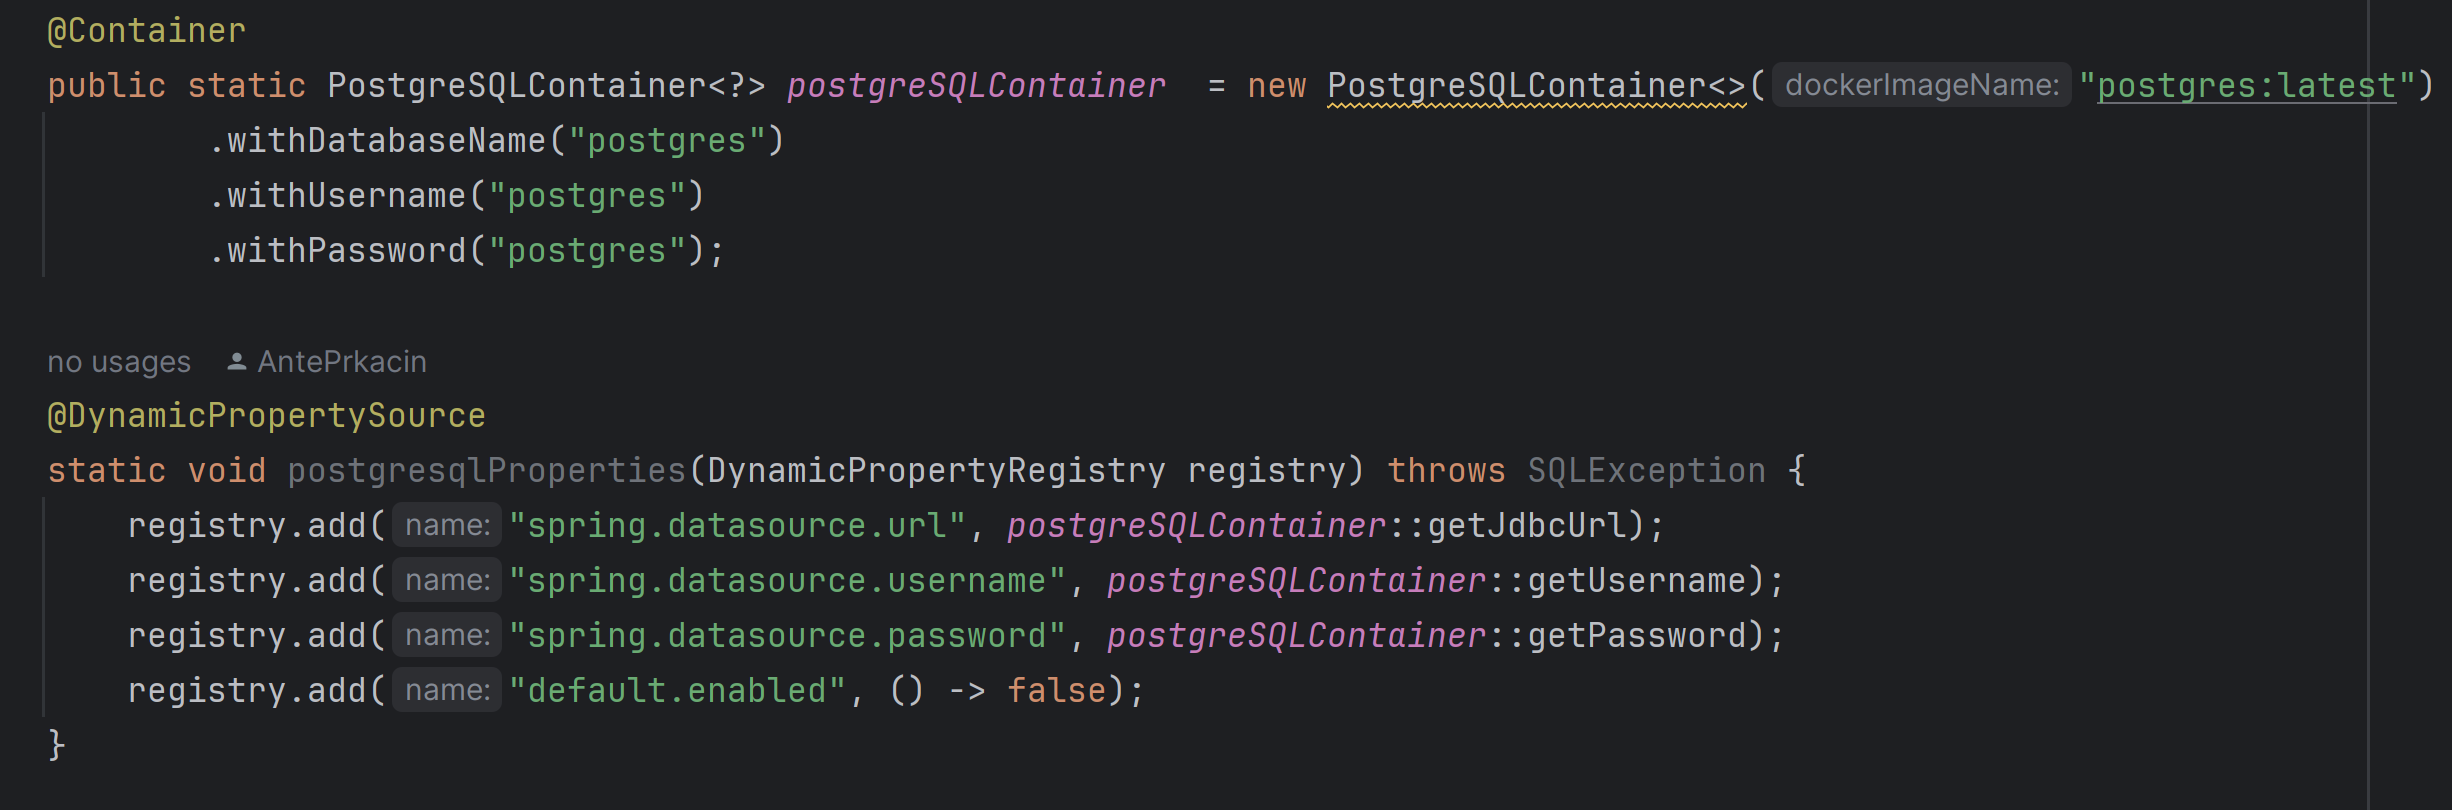
\includegraphics[scale=0.60]{slike/IT_containerized_docker.png}
                \centering
                \caption{Dizanje baze u integracijskom testu}
                \label{fig:IT_docker}
            \end{figure}

            Nakon što se baza digne, a prije pokretanja testova, izvršava se funkcija s anotacijom @BeforeEach koja u bazu umeće podatke potrebne za testiranje.
            Na primjer, ako se testira metoda za brisanje prijave, u bazu će se prije tog testa umetnuti jedna prijava.
			Ova funkcija se izvršava prije svakog testa.
            Umetanje u bazu funkcionira tako da se napravi String varijabla koja je jednaka SQL naredbi.
			Potom se izgradi objekt koji se želi umetnuti u bazu i u SQL naredbu se upisuju atributi tog objekta.
			Na kraju se SQL naredba izvršava i podatak se upisuje u bazu (Slika \ref{fig:beforeEach}).
            \begin{figure}[H]
                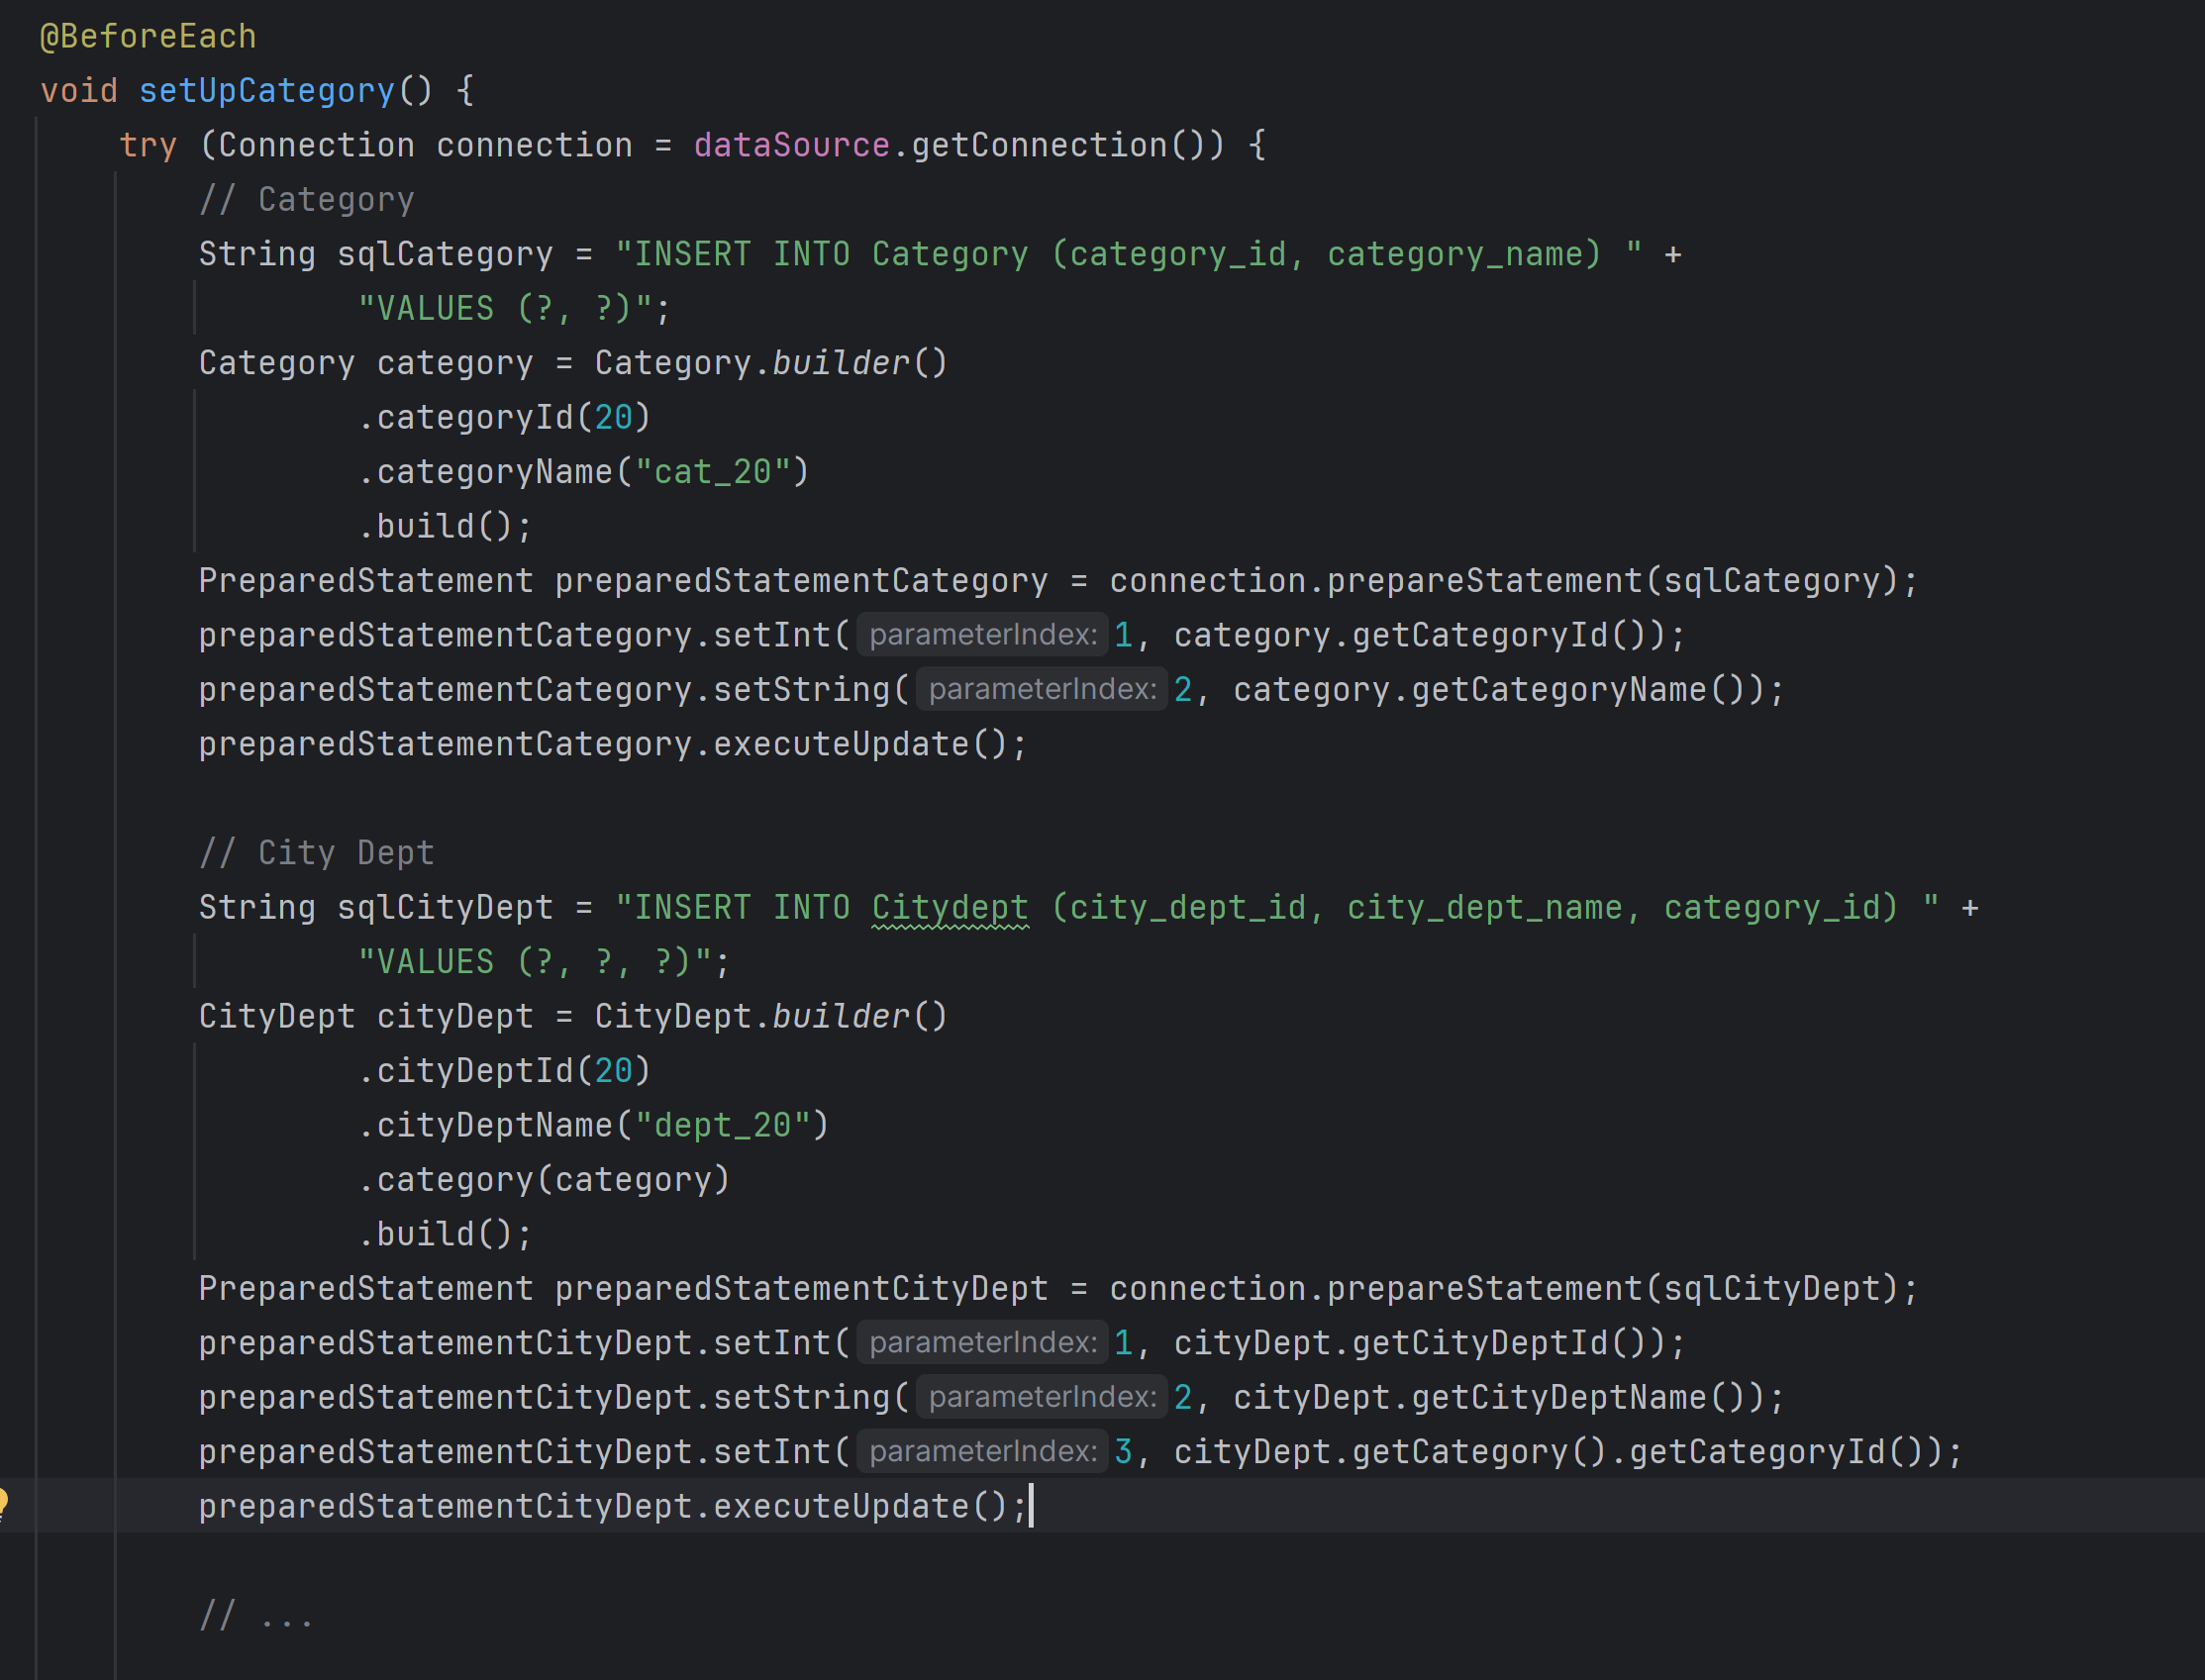
\includegraphics[scale=0.60]{slike/IT_beforeEach.png}
                \centering
                \caption{Umetanje podataka u bazu}
                \label{fig:beforeEach}
            \end{figure}

            Testovi su funkcije s anotacijom @Test.
			Za testiranje se koristi mockMvc.perform() funkcija koja simulira HTTP zahtjev, definira HTTP metodu za poziv API-a,
            predaje JSON ako treba, definira kakav contentType treba predati, je li potreban jwt za pristup API-ju i
			koji HTTP status se očekuje kao odgovor tog zahtjeva (slika \ref{fig:test}).
            \begin{figure}[H]
                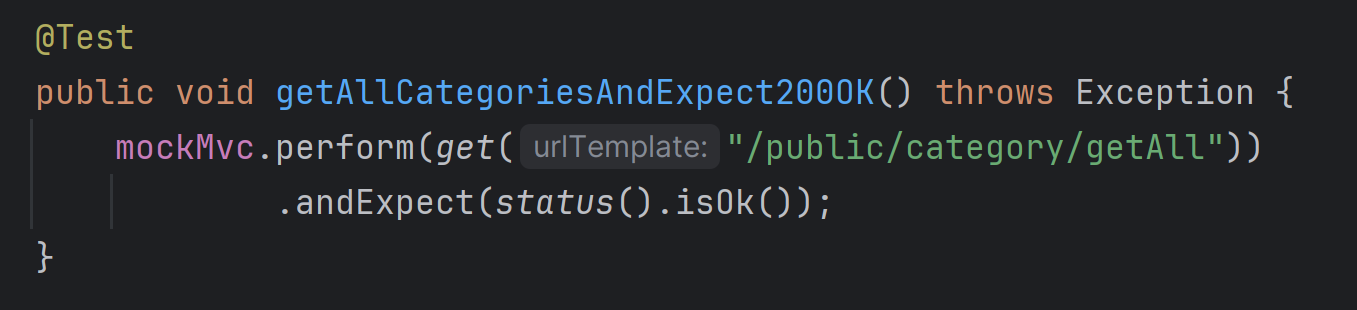
\includegraphics[scale=0.60]{slike/IT_test.png}
                \centering
                \caption{Integracijski test}
                \label{fig:test}
            \end{figure}

            Po završetku svakog testa izvršava se funkcija s anotacijom @AfterEach.
			Ona koristi JdbcTestUtils.deleteFromTables() funkciju kako bi izbrisala sve podatke iz određene tablice u bazi.
			Na ovakav način se osigurava da ako se nešto umetne u bazu prilikom testa,
			poslije završetka testa će se i izbrisati (slika \ref{fig:afterEach}).
            \begin{figure}[H]
                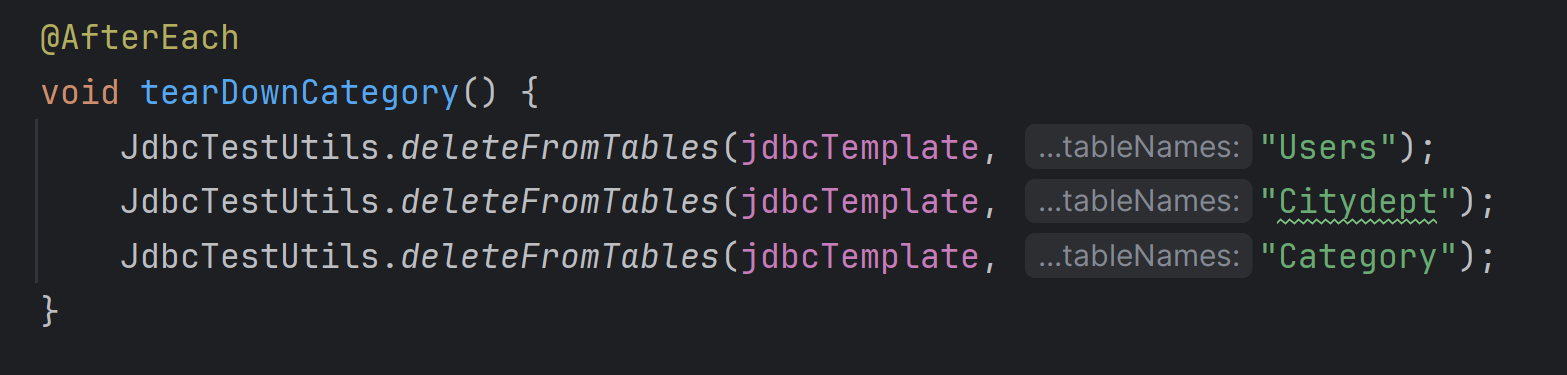
\includegraphics[scale=0.60]{slike/IT_afterEach.png}
                \centering
                \caption{Brisanje podataka iz baze nakon testa}
                \label{fig:afterEach}
            \end{figure}

            \eject
			
			
			
			\subsection{Ispitivanje sustava}

			Ispitivanje funkcionalnosti sustava je provedeno pomoću Selenium testova
			pisanih i jeziku JavaScript uz preglednik Google Chrome. Ukupno je napisano
			8 testova od kojih 3 provjerava kako se sustav nosi s pogrešnim unosima.
			 \\
			\textbf{1. Ispitni slučaj: Prijava korisnika}
			 \begin{itemize}
				\item \textbf{Ulaz:} Email adresa i lozinka korisnika 
				\item \textbf{Očekivani izlaz:} Nakon prijave nalazit ćemo se na početnoj stranici s korisničkim imenom prikazanim u gornjem desnom kutu.
				\item \textbf{Koraci:} 
				\\ 1. Klik na gumb Login/Register
				\\ 2. Unos korisničkih podataka, točnije emaila i lozinke
				\\ 3. Klik na gumb Prijava
			\end{itemize}

			\begin{verbatim}
				const { By, Key, Builder, until } = require("selenium-webdriver");

				async function prijava() {
				let driver = await new Builder().forBrowser("chrome").build();
				try {
					await driver.get("https://cestafix-fe.onrender.com/");
					const buttonElement = await driver.findElement(By.css('#login'));
					await buttonElement.click();
					const usernameField = await driver.findElement(By.css('#username'));
					await usernameField.sendKeys('filip.simunovic@gmail.com');
					const passwordField = await driver.findElement(By.css('#password'));
					await passwordField.sendKeys('Simiklimi.5');
					const submitButton = await driver.findElement(By.css('#submit'));
					await submitButton.click();
					await driver.sleep(10000);
				} catch (error) {
					console.error("Test failed:", error);
				} finally {
					// Quit the driver
					console.log("Test je prosao uspjesno.");
					await driver.quit();
				}
				}

				prijava();
			\end{verbatim}

			\textbf{2. Ispitni slučaj: Registracija korisnika}
			 \begin{itemize}
				\item \textbf{Ulaz:} Ime, prezime, email i lozinka korisnika
				\item \textbf{Očekivani izlaz:} Nakon uspješne registracije nalazit ćemo se na početnoj stranici s korisničkim imenom prikazanim u gornjem desnom kutu.
				\item \textbf{Koraci:} 
				\\ 1. Klik na gumb Login/Register
				\\ 2. Klik na link "Nemaš račun? Registriraj se!"
				\\ 3. Unos korisničkih podataka
				\\ 4. Klik na gumb Registriraj se
			\end{itemize}

			\begin{verbatim}
				const { By, Key, Builder, until } = require("selenium-webdriver");


				async function register() {
					let driver = await new Builder().forBrowser("chrome").build();
				  try {
					await driver.get("https://cestafix-fe.onrender.com/");
					const buttonElement = await driver.findElement(By.css('#login'));
					await buttonElement.click();
					const registerElement = await driver.findElement(By.css('#nemaracun'));
					await registerElement.click();
					const imeField = await driver.findElement(By.css('#imeid'));
					await imeField.sendKeys('Da');
					const prezimeField = await driver.findElement(By.css('#prezimeid'));
					await prezimeField.sendKeys('Vinki');
					const emailField = await driver.findElement(By.css('#emailid'));
					await emailField.sendKeys('da.vinki@gmail.com');
					const passwordField = await driver.findElement(By.css('#passwordid'));
					await passwordField.sendKeys('Vinki.66');
					const passwordrepeatField = await driver.findElement(By.css('#repatpasswordid'));
					await passwordrepeatField.sendKeys('Vinki.66');
					const submitField = await driver.findElement(By.css('#signupid'));
					await submitField.click();
					await driver.sleep(10000);
				  } catch (error) {
					console.error("Test failed:", error);
				  } finally {
					// Quit the driver
					console.log("Test je prosao uspjesno.");
					await driver.quit();
				  }
				
				}
				
				register();				
			\end{verbatim}

			\textbf{3. Ispitni slučaj: Neuspjela prijava korisnika}
			 \begin{itemize}
				\item \textbf{Ulaz:} Email adresa i \textit{netočna} lozinka korisnika
				\item \textbf{Očekivani izlaz:} Nakon unosa pogrešne lozinke korisniku se trebaju ispisati da su uneseni krivi podatci u istom prozoru.
				\item \textbf{Koraci:} 
				\\ 1. Klik na gumb Login/Register
				\\ 2. Unos korisničnih podataka, točnije emaila i lozinke
				\\ 3. Klik na gumb Prijava
			\end{itemize}

			\begin{verbatim}
				const { By, Key, Builder, until } = require("selenium-webdriver");

				async function prijava() {
				let driver = await new Builder().forBrowser("chrome").build();
				try {
					await driver.get("https://cestafix-fe.onrender.com/");
					const buttonElement = await driver.findElement(By.css('#login'));
					await buttonElement.click();
					const usernameField = await driver.findElement(By.css('#username'));
					await usernameField.sendKeys('filip.simunovic@gmail.com');
					const passwordField = await driver.findElement(By.css('#password'));
					await passwordField.sendKeys('Simiklimiii.5');
					const submitButton = await driver.findElement(By.css('#submit'));
					await submitButton.click();
					await driver.sleep(10000);
				} catch (error) {
					console.error("Test failed:", error);
				} finally {
					// Quit the driver
					console.log("Test je prosao uspjesno.");
					await driver.quit();
				}
				}

			prijava();
			\end{verbatim}

			\textbf{4. Ispitni slučaj: Registracija korisnika i brisanje računa}
			 \begin{itemize}
				\item \textbf{Ulaz:} Ime, prezime, email i lozinka korisnika
				\item \textbf{Očekivani izlaz:} Nakon registriranja i brisanja računa, ako se pokušamo logirati s istim podatcima dobit ćemo neuspjelu prijavu.
				\item \textbf{Koraci:} 
				\\ 1. Klik na gumb Login/Register
				\\ 2. Klik na link "Nemaš račun? Registriraj se!"
				\\ 3. Unos korisničnih podataka
				\\ 4. Klik na gumb Registriraj se
				\\ 5. Klik na gumb koji prikazuje ime korisnika
				\\ 6. Klik na gumb Pobriši račun!!!
				\\ 7. Klik na gumb POTVRDI
				\\ 8. Klik na gumb Login/Register
				\\ 9. Unos korisničnih podataka
				\\ 10. Klik na gumb Prijava
			\end{itemize}

			\begin{verbatim}
				const { By, Key, Builder, until } = require("selenium-webdriver");

				async function register() {
					let driver = await new Builder().forBrowser("chrome").build();
				try {
					await driver.get("https://cestafix-fe.onrender.com/");
					const buttonElement = await driver.findElement(By.css('#login'));
					await buttonElement.click();
					const registerElement = await driver.findElement(By.css('#nemaracun'));
					await registerElement.click();
					const imeField = await driver.findElement(By.css('#imeid'));
					await imeField.sendKeys('Da');
					const prezimeField = await driver.findElement(By.css('#prezimeid'));
					await prezimeField.sendKeys('Vinki');
					const emailField = await driver.findElement(By.css('#emailid'));
					await emailField.sendKeys('da.vinkiiiiiiiii@gmail.com');
					const passwordField = await driver.findElement(By.css('#passwordid'));
					await passwordField.sendKeys('Vinkii.66');
					const passwordrepeatField = await driver.findElement
					(By.css('#repatpasswordid'));
					await passwordrepeatField.sendKeys('Vinkii.66');
					const submitField = await driver.findElement(By.css('#signupid'));
					await submitField.click();
					await driver.sleep(5000);
					const accountField = await driver.findElement(By.css("#account"));
					await accountField.click();
					await driver.sleep(2000);
					const deleteField = await driver.findElement(By.css("#brisiid"));
					await deleteField.click();
					await driver.sleep(2000);
					const delete2Field = await driver.findElement(By.css("#brisiaccid"));
					await delete2Field.click();
					await driver.sleep(2000);
					const loginButtonElement = await driver.findElement(By.css('#login'));
					await loginButtonElement.click();
					const username2Field = await driver.findElement(By.css('#username'));
					await username2Field.sendKeys('da.vinkiiiiiiiii@gmail.com');
					const password2Field = await driver.findElement(By.css('#password'));
					await password2Field.sendKeys('Vinkii.66');
					const submit2Button = await driver.findElement(By.css('#submit'));
					await submit2Button.click();
					await driver.sleep(5000);
				} catch (error) {
					console.error("Test failed:", error);
				} finally {
					// Quit the driver
					console.log("Test je prosao uspjesno.");
					await driver.quit();
				}
				}
				register();
			\end{verbatim}

			\textbf{5. Ispitni slučaj: Prijava štete anonimnog korisnika}
			 \begin{itemize}
				\item \textbf{Ulaz:} Naziv štete, opis štete, adresa štete
				\item \textbf{Očekivani izlaz:} Nakon uspješne prijave izbacit će se prozor da id-jem prijave pomoću kojeg možemo pratiti istu.
				\item \textbf{Koraci:} 
				\\ 1. Klik na gumb Prijavi Štetu!
				\\ 2. Unos podataka prijave
				\\ 3. Klik na gumb Submit
			\end{itemize}

			\begin{verbatim}
				const { By, Key, Builder, until } = require("selenium-webdriver");

				async function prijava() {
				let driver = await new Builder().forBrowser("chrome").build();
				try {
					await driver.get("https://cestafix-fe.onrender.com/");
					const buttonElement = await driver.findElement(By.css('#prijava'));
					await buttonElement.click();
					const nameField = await driver.findElement(By.css('#name'));
					await nameField.sendKeys('Palo stup na kolnik');
					const descriptionField = await driver.findElement(By.css('#description'));
					await descriptionField.sendKeys('Pao STOP znak tamo di hodaju ljudi');
					const addressField = await driver.findElement(By.css('#address'));
					await addressField.sendKeys('Unska 4');
					const submitButton = await driver.findElement(By.css('.confirmButton'));
					await submitButton.click();
					await driver.sleep(40000);
					const confirmButton = await driver.findElement(By.css('.loginbtn'));
					await confirmButton.click();
				} catch (error) {
					console.error("Test failed:", error);
				} finally {
					// Quit the driver
					console.log("Test je prosao uspjesno.");
					await driver.quit();
				}
				}
				prijava();
			\end{verbatim}


			\textbf{6. Ispitni slučaj: Prijava štete prijavljenog korisnika}
			 \begin{itemize}
				\item \textbf{Ulaz:} Email adresa i lozinka korisnika, naziv štete, opis štete, adresa štete
				\item \textbf{Očekivani izlaz:} Nakon uspješne prijave izbacit će se prozor da id-jem prijave pomoću kojeg možemo pratiti istu.
				\item \textbf{Koraci:} 
				\\ 1. Klik na gumb Login/Register
				\\ 2. Unos korisničnih podataka
				\\ 3. Klik na gumb Prijava
				\\ 4. Klik na gumb Prijavi Štetu!
				\\ 5. Unos podataka prijave
				\\ 6. Klik na gumb Submit
			\end{itemize}

			\begin{verbatim}
				const { By, Key, Builder, until } = require("selenium-webdriver");

				async function prijava() {
				let driver = await new Builder().forBrowser("chrome").build();
				try {
					await driver.get("https://cestafix-fe.onrender.com/");
					const buttonElement = await driver.findElement(By.css('#login'));
					await buttonElement.click();
					const usernameField = await driver.findElement(By.css('#username'));
					await usernameField.sendKeys('filip.simunovic@gmail.com');
					const passwordField = await driver.findElement(By.css('#password'));
					await passwordField.sendKeys('Simiklimi.5');
					const submitButton = await driver.findElement(By.css('#submit'));
					await submitButton.click();
					await driver.sleep(5000);
					// prijava
					const button2Element = await driver.findElement(By.css('#prijava'));
					await button2Element.click();
					const nameField = await driver.findElement(By.css('#name'));
					await nameField.sendKeys('Palo stup na kolnik opet');
					const descriptionField = await driver.findElement(By.css('#description'));
					await descriptionField.sendKeys('Pao js jedan 
					STOP znak tamo di hodaju ljudi');
					const addressField = await driver.findElement(By.css('#address'));
					await addressField.sendKeys('Unska 5');
					const submit2Button = await driver.findElement(By.css('.confirmButton'));
					await submit2Button.click();
					await driver.sleep(40000);
				} catch (error) {
					console.error("Test failed:", error);
				} finally {
					// Quit the driver
					console.log("Test je prosao uspjesno.");
					await driver.quit();
				}
				}

				prijava();
			\end{verbatim}


			
			\textbf{7. Ispitni slučaj: Neuspjela registracija korisnika}
			 \begin{itemize}
				\item \textbf{Ulaz:} Ime, prezime, email i \text{neispravna lozinka} (ne zadovoljava uvjet da mora biti dugačka 8 znakova, imati jedno veliko, jedno malo slovo, jedan broj i jedan specijalan znak) korisnika
				\item \textbf{Očekivani izlaz:} Nakon neuspješne registracije korisniku će se ispitati kako lozinka ne zadovoljava sigurnosni uvjet.
				\item \textbf{Koraci:} 
				\\ 1. Klik na gumb Login/Register
				\\ 2. Klik na link "Nemaš račun? Registriraj se!"
				\\ 3. Unos korisničnih podataka
				\\ 4. Klik na gumb Registriraj se
			\end{itemize}

			\begin{verbatim}
					const { By, Key, Builder, until } = require("selenium-webdriver");

				// Test sa neispravnom lozinkom
				async function register() {
					let driver = await new Builder().forBrowser("chrome").build();
				try {
					await driver.get("https://cestafix-fe.onrender.com/");
					const buttonElement = await driver.findElement(By.css('#login'));
					await buttonElement.click();
					const registerElement = await driver.findElement(By.css('#nemaracun'));
					await registerElement.click();
					const imeField = await driver.findElement(By.css('#imeid'));
					await imeField.sendKeys('Da');
					const prezimeField = await driver.findElement(By.css('#prezimeid'));
					await prezimeField.sendKeys('Vinki');
					const emailField = await driver.findElement(By.css('#emailid'));
					await emailField.sendKeys('da.vinki@gmail.com');
					const passwordField = await driver.findElement(By.css('#passwordid'));
					await passwordField.sendKeys('Vinki.5');
					const passwordrepeatField = await driver.findElement
					(By.css('#repatpasswordid'));
					await passwordrepeatField.sendKeys('Vinki.5');
					const submitField = await driver.findElement(By.css('#signupid'));
					await submitField.click();
					await driver.sleep(10000);
				} catch (error) {
					console.error("Test failed:", error);
				} finally {
					// Quit the driver
					console.log("Test je prosao uspjesno.");
					await driver.quit();
				}
				}
				register();
			\end{verbatim}

			\textbf{8. Ispitni slučaj: Neuspjela prijava štete logiranog korisnika}
			 \begin{itemize}
				\item \textbf{Ulaz:} Podatci prijave \textit{bez} podatka o lokaciji
				\item \textbf{Očekivani izlaz:} Nakon što nije unesena nikakva lokacija, korisniku će se u prozoru prikazati ispis "Došlo je do greške, provjerite unos adrese prijave!"
				\item \textbf{Koraci:} 
				\\ 1. Klik na gumb Login/Register
				\\ 2. Unos korisničnih podataka
				\\ 3. Klik na gumb Prijava
				\\ 4. Klik na gumb Prijavi Štetu!
				\\ 5. Unos podataka prijave
				\\ 6. Klik na gumb Submit
			\end{itemize}

			\begin{verbatim}
				const { By, Key, Builder, until } = require("selenium-webdriver");

			// report bez unosa lokacije - error
			async function prijava() {
			let driver = await new Builder().forBrowser("chrome").build();
			try {
				await driver.get("https://cestafix-fe.onrender.com/");
				const buttonElement = await driver.findElement(By.css('#login'));
				await buttonElement.click();
				const usernameField = await driver.findElement(By.css('#username'));
				await usernameField.sendKeys('filip.simunovic@gmail.com');
				const passwordField = await driver.findElement(By.css('#password'));
				await passwordField.sendKeys('Simiklimi.5');
				const submitButton = await driver.findElement(By.css('#submit'));
				await submitButton.click();
				await driver.sleep(5000);
				// prijava
				const button2Element = await driver.findElement(By.css('#prijava'));
				await button2Element.click();
				const nameField = await driver.findElement(By.css('#name'));
				await nameField.sendKeys('Palo stup na kolnik opet');
				const descriptionField = await driver.findElement(By.css('#description'));
				await descriptionField.sendKeys('Pao js jedan STOP znak tamo di hodaju ljudi');
				const submit2Button = await driver.findElement(By.css('.confirmButton'));
				await submit2Button.click();
				await driver.sleep(40000);
			} catch (error) {
				console.error("Test failed:", error);
			} finally {
				// Quit the driver
				console.log("Test je prosao uspjesno.");
				await driver.quit();
			}
			}
			prijava();
			\end{verbatim}

			
			\eject 
		
		\section{Dijagram razmještaja}

			Dijagram razmještaja opisuje topologiju sustava i usredotočen je na odnos sklopovskih i programskih
			dijelova. Prikazan je na slici 5.1. Na poslužiteljskom računalu se nalazi Render servis, Frontend HTTP poslužitelj, Backend HTTP 
			poslužitelj te PostgreSQL poslužitelj na kojem je baza podataka. Na Frontend HTTP poslužitelju se nalazi
			React frontend CestaFix aplikacije. Na Backend HTTP poslužitelju se nalazi ReportApplication.jar, tj. 
			Java Archive file u kojem se nalazi \textit{backend} CestaFix aplikacije. Poslužiteljska strana aplikacije
			ostvarena je pomoću servisa Render. Klijenti koriste web preglednik kako bi pristupili web aplikaciji. 
			Sustav je baziran na arhitekturi "klijent - poslužitelj", a komunikacija između računala korisnika
			i poslužitelja odvija se preko HTTP veze.

			\begin{figure}[H]
				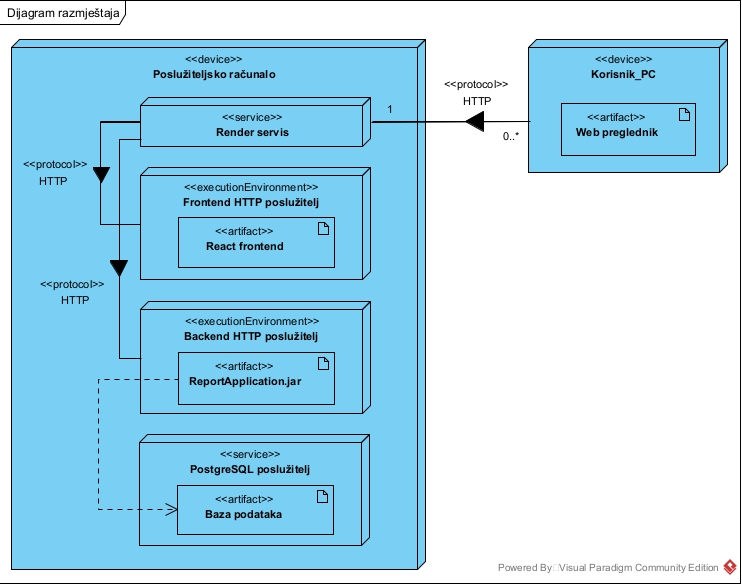
\includegraphics[scale=0.60]{slike/DR.jpg} %veličina slike u odnosu na originalnu datoteku i pozicija slike
				\centering
				\caption{Dijagram razmještaja}
				\label{fig:DijagramRazmjestaja}
			\end{figure}

			\eject 
		
			\section{Upute za puštanje u pogon}

			Za pogon naše aplikacije korištena je platforma Render koja pruža besplatno puštanje aplikacije u pogon sa, naravno, ograničenim mogućnostima.   

			\subsection{Puštanje baze podataka u pogon} 
			Prvo je potrebno upogoniti bazu podataka. Nakon prijavljivanja u platformu, potrebno je odabrati opciju New \texttt{->} PostgreSQL  (Slika \ref{fig:Kreiranjenovogservisa}). 
			Zatim je na ekranu prikazan unos podataka za bazu podataka, za što smo mi ostavili sve prazno (automatski se generira) osim imena servisa, te je za regiju potrebno postaviti \texttt{Frankfurt(EU Central)} (Slika \ref{fig:Unos podataka za bazu}).
			Nedostatak besplatne verzije Rendera je to što je moguća samo jedna baza podataka koja je ograničena na trajanje od 3 mjeseca, no to je dovoljno za naše potrebe.
			\begin{figure}[H]
				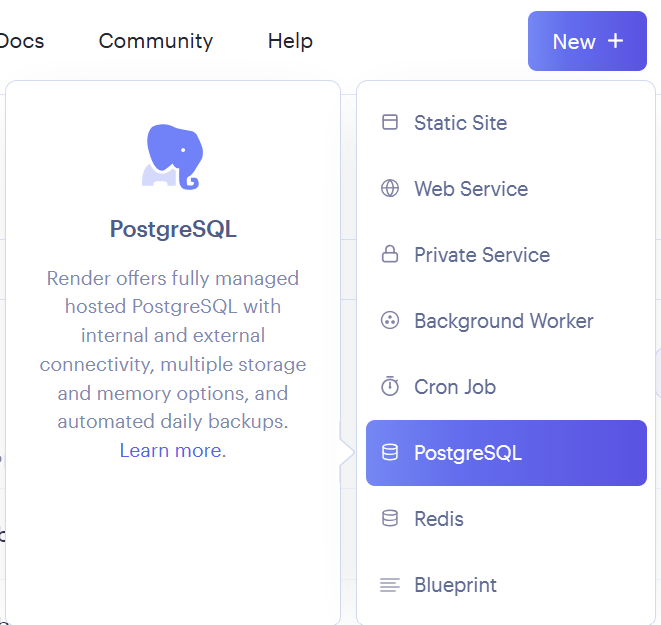
\includegraphics[scale=0.60]{slike/render1.png} %veličina slike u odnosu na originalnu datoteku i pozicija slike
				\centering
				\caption{Kreiranje novog servisa}
				\label{fig:Kreiranjenovogservisa}
			\end{figure}

			\begin{figure}[H]
				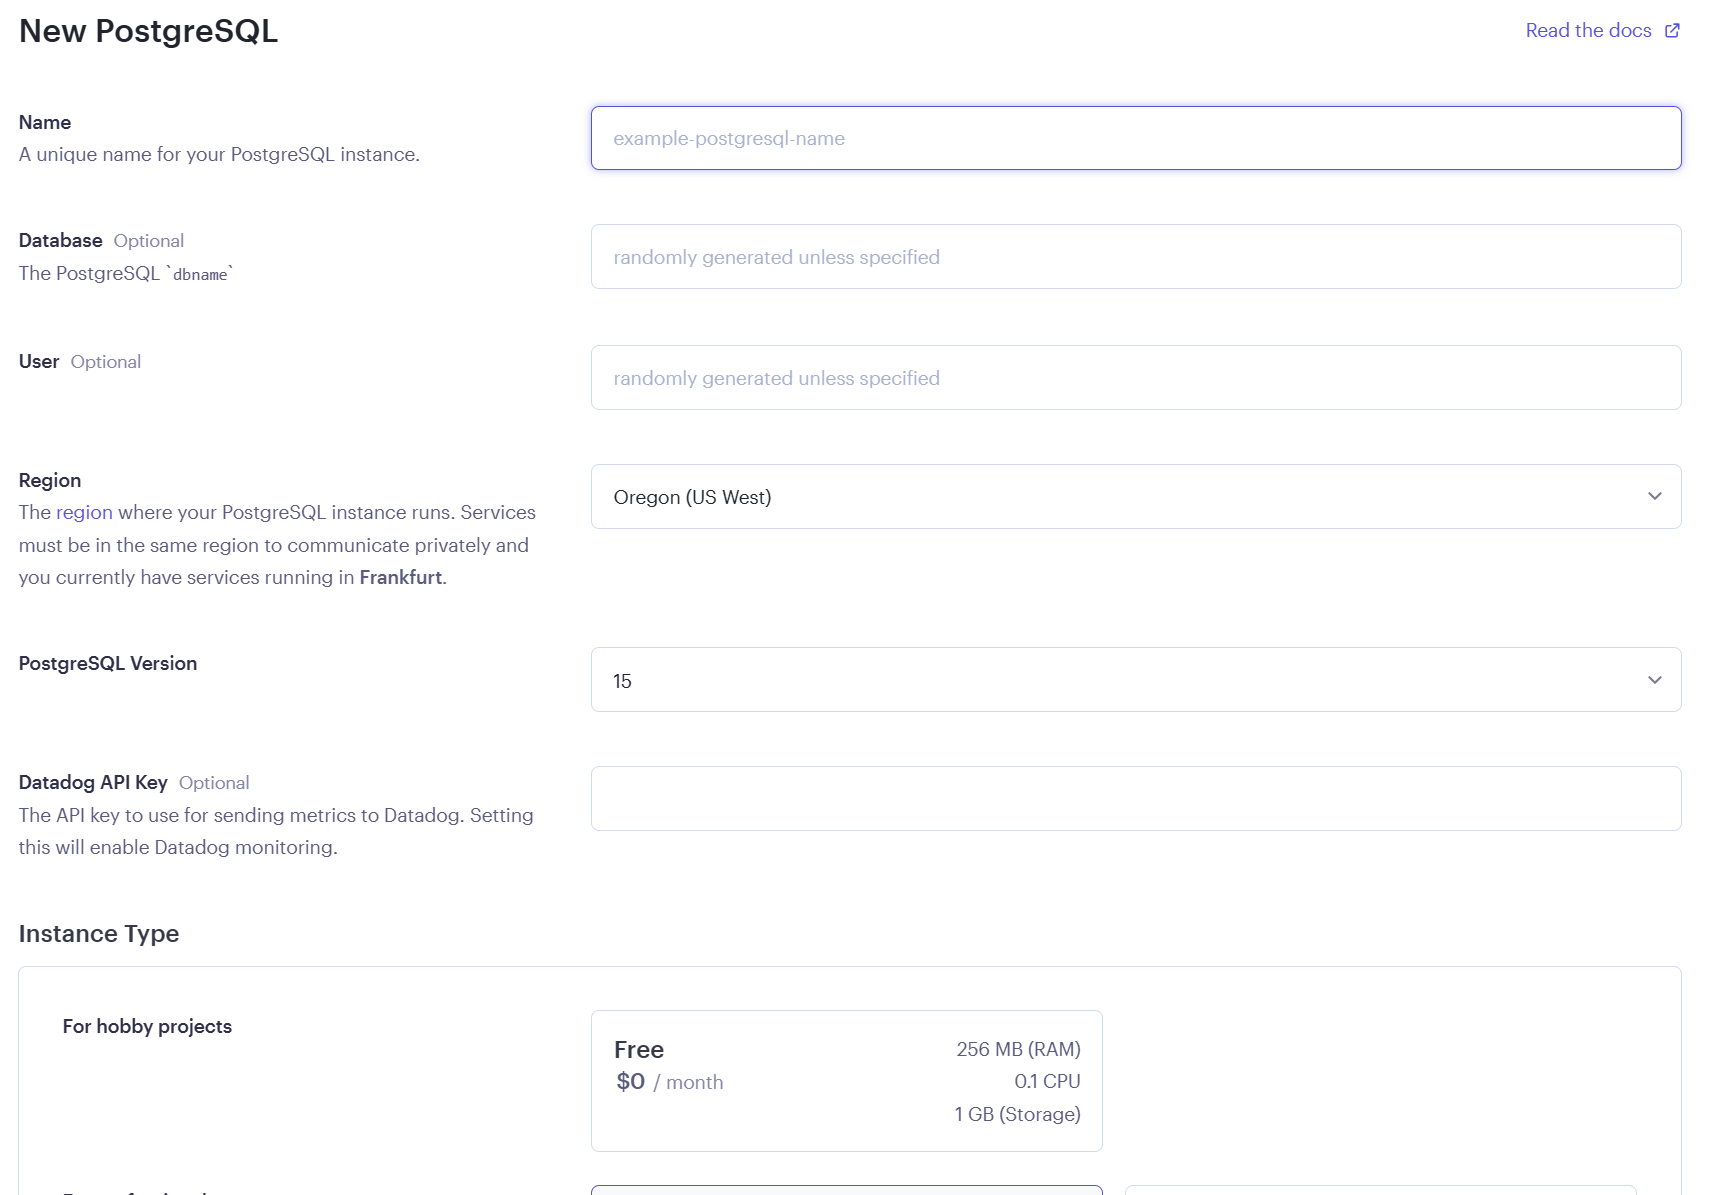
\includegraphics[scale=0.40]{slike/render2.png} %veličina slike u odnosu na originalnu datoteku i pozicija slike
				\centering
				\caption{Unos podataka za bazu}
				\label{fig:Unos podataka za bazu}
			\end{figure}

			\subsection{Puštanje backenda u pogon} 
			Isto tako je potrebno podesiti \textit{backend}. Prvo je potrebno odabrati opciju \texttt{Web Service} u \ref{fig:Kreiranjenovogservisa}.
			Nakon toga imamo opciju odabrati deploy preko github repozitorija, što omogućava automatsko redeployanje svaki put kada se napravi novi commit.
			Nakon odabira našeg repozitorija, opet imamo ekran za unos podataka \ref{fig:UnosPodatakaZaBack}
			\begin{figure}[H]
				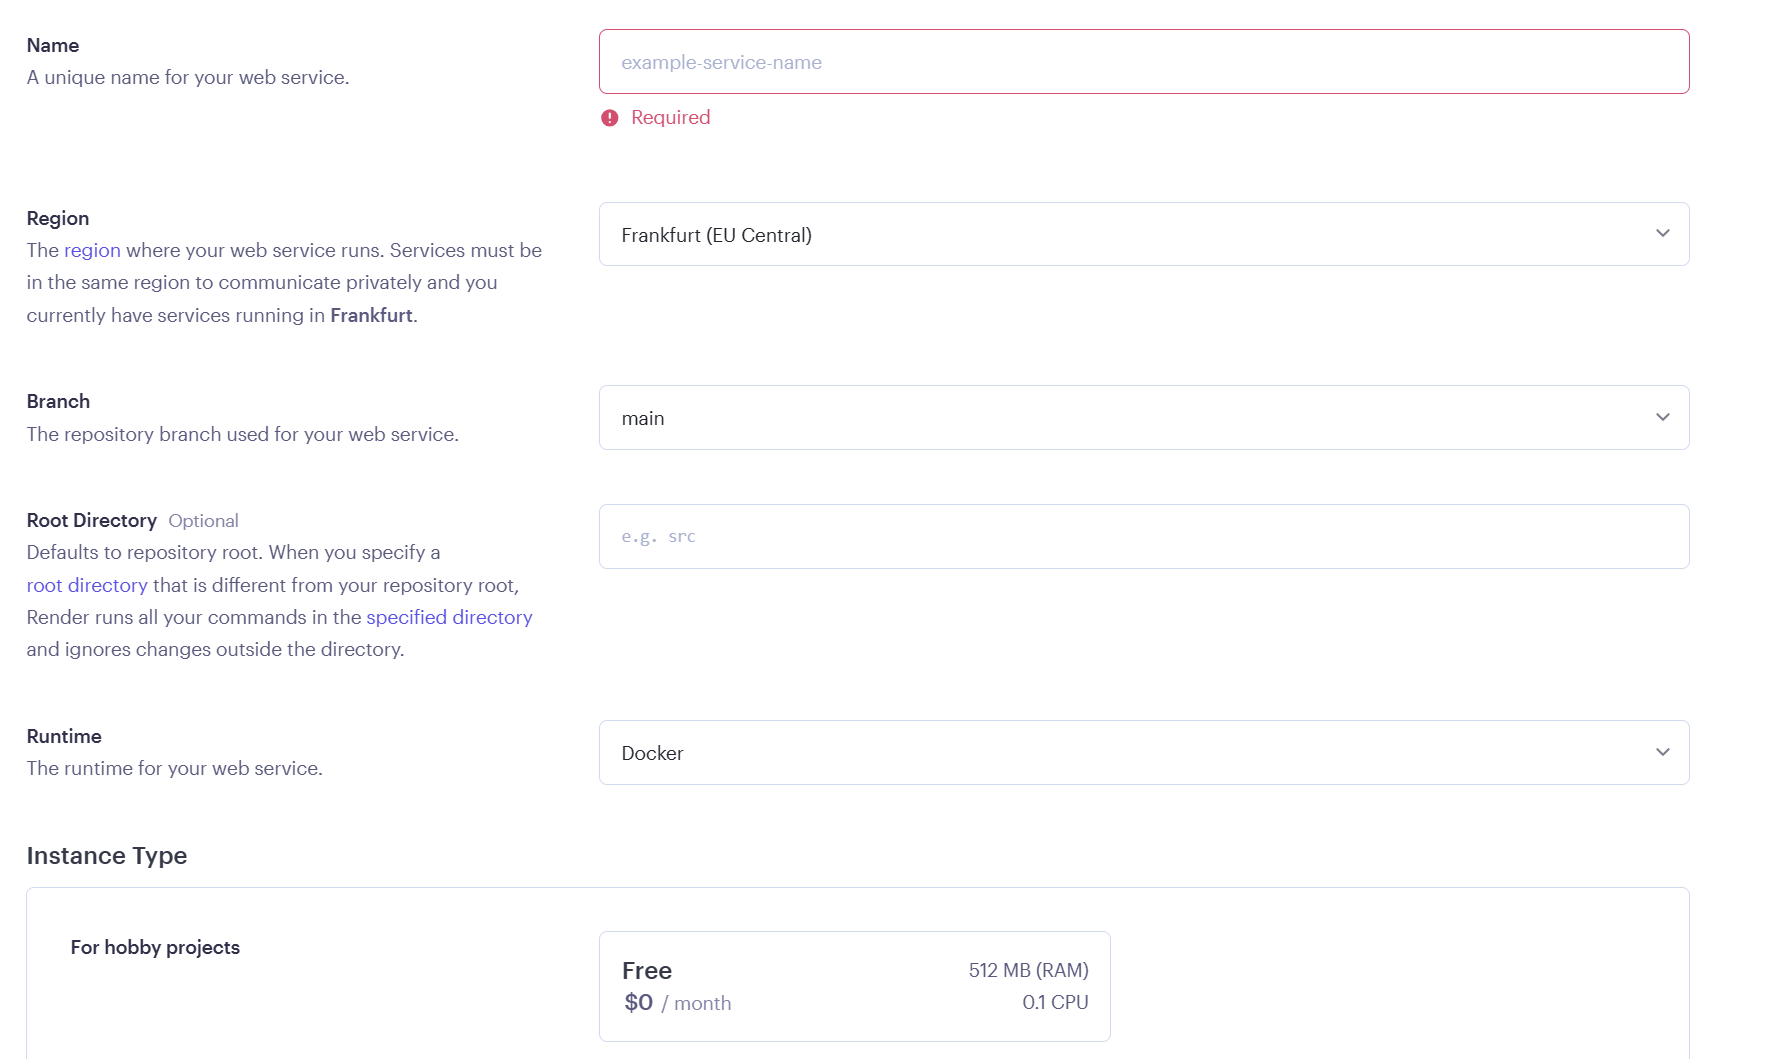
\includegraphics[scale=0.40]{slike/render3.png} %veličina slike u odnosu na originalnu datoteku i pozicija slike
				\centering
				\caption{Unos podataka za backend}
				\label{fig:UnosPodatakaZaBack}
			\end{figure}
			Za ime upisati željeno ime servisa, za regiju staviti Frankfurt, odabrati granu i pozicionirati se u \textit{backend} direktorij. Za runtime staviti Docker.
			Nakon toga je potrebno upisat podatke za varijable okoline koje nam omogućavaju povezivanje na prethodno deployanu bazu \ref{fig:EnvVarijable}
			\begin{figure}[H]
				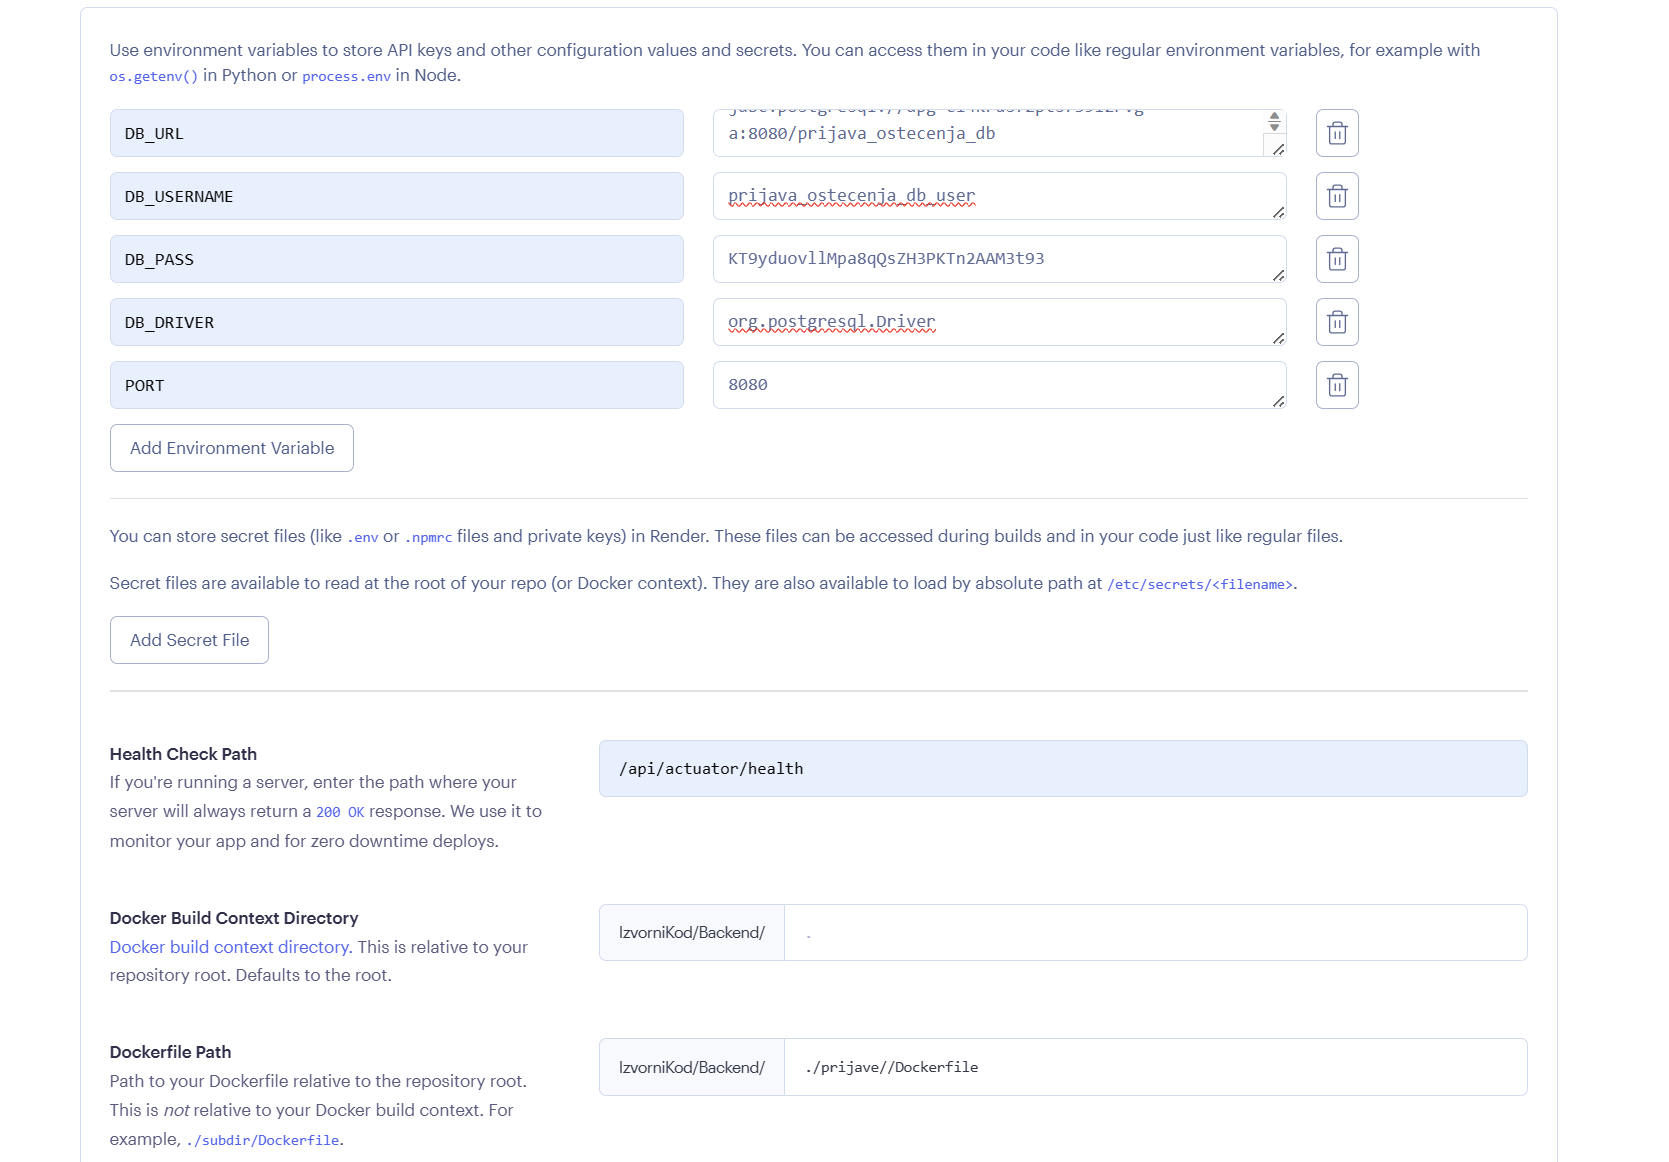
\includegraphics[scale=0.40]{slike/render4.png} %veličina slike u odnosu na originalnu datoteku i pozicija slike
				\centering
				\caption{Unos varijabli okoline za backend}
				\label{fig:EnvVarijable}
			\end{figure}

			

			\eject 
\chapter{Zaključak i budući rad}
		
		Zadatak našeg tima bio je razvoj aplikacije za prijavu štete javnih površina. Aplikacija je trebala olakšati 
		prijavu oštećenja javnih površina i cesta u gradovima i Provedba projekta bila je u dvije faze.

		Prva faza projekta uključivala je formiranje tima za razvoj aplikacije, dodjelu projektnog zadatka i intenzivan
		rad na dokumentiranju zahtjeva. Kvalitetnom provedbom prve faze uvelike je olakšan daljnji rad na razvoju 
		osmišljene aplikacije. Izrađeni obrasci i dijagrami (obrasci uporabe, sekvencijski dijagrami, model baze podataka,
		dijagrami razreda) omogućili su razvojnim timovima za \textit{frontend} i \textit{backend} lakši rad i organizaciju.
		Izrada vizualnog koncepta aplikacije uštedila je mnogo vremena u drugoj fazi razvoja, gdje je služila kao idejni 
		temelj za razvoj. Tijekom prve faze projekta ostvarene su osnovne funkcionalnosti aplikacije.

		Druga faza projekta bila je kraća, ali puno intenzivnija u razvoju aplikacije. Nedostatak iskustva članova u izradi
		sličnih projekata bio je izazov, no kroz projekt članovi tima imali su priliku upoznati i savladati razne alate i 
		programske jezike kako bi uspješno realizirali projekt. Uz tehničke vještine članovi su imali priliku razvijati 
		organizacijske vještine. Tijekom druge faze izrađeni su novi dijagrami (dijagram stanja, dijagram aktivnosti, dijagram
		komponenti, dijagram razmještaja) te unaprijeđeni već postojeći dijagrami (model baze podataka, dijagrami razreda).
		Dobro izrađen kostur projekta uštedio nam je mnogo vremena prilikom izrade aplikacije. Tijekom druge faze projekta ostvarena 
		je većina funkcionalnosti aplikacije.

		Tijekom projekta uspjeli smo realizirati većinu zamišljenih funkcionalnosti. One se odnose na funkcionalnosti za 
		neregistriranog korisnika i registriranog korisnika koji se dijeli na građanina i službenika gradskog ureda. Time 
		smo ostvarili sve tražene funkcionalnosti zadane u projektnom zadatku. Iznimka od toga je obrazac uporabe UC20 koji se 
		odnosi na ponovno postavljanje zaboravljene lozinke. Spomenuti obrazac uporabe nije zamišljen u projektnom zadatku nego
		kao ideja za korisnu funkcionalnost u aplikaciji, stoga zbog vremenske ograničenosti preostaje za budući rad na aplikaciji.
		Funkcionalnosti administratora također nam preostaju za budući rad. Konkretno je riječ o obrascima uporabe UC04, UC05,
		UC06, UC18, UC19, UC21, UC22 i UC23. U trenutnoj verziji aplikacije one se ostvaruju ručno u bazi podataka. 

		Informiranost članova o napretku projekta ostvarili smo korištenjem aplikacije Discord i sastancima uživo. Svi 
		članovi pokazali su zainteresiranost za projekt čime je rad bio ugodan i bez organizacijskih problema. Zadovoljni smo s
		realiziranom aplikacijom i zajedničkim radom na projektu.

		\eject 
\chapter*{Popis literature}
		\addcontentsline{toc}{chapter}{Popis literature}
	 	
 		\textbf{\textit{Kontinuirano osvježavanje}}
	
		\textit{Popisati sve reference i literaturu koja je pomogla pri ostvarivanju projekta.}
		
		
		\begin{enumerate}
			
			
			\item  Programsko inženjerstvo, FER ZEMRIS, \url{http://www.fer.hr/predmet/proinz}
			
			\item  I. Sommerville, "Software engineering", 8th ed, Addison Wesley, 2007.
			
			\item  T.C.Lethbridge, R.Langaniere, "Object-Oriented Software Engineering", 2nd ed. McGraw-Hill, 2005.
			
			\item  I. Marsic, "Software engineering book", Department of Electrical and Computer Engineering, Rutgers University, \url{http://www.ece.rutgers.edu/~marsic/books/SE}
			
			\item  Visual Paradigm, \url{https://www.visual-paradigm.com/}
			
			\item  Tehničko predavanje o backendu, \url{https://gitlab.com/hrvojesimic/progi-project-teams-backend/}

		\end{enumerate}
		
		 


\begingroup
\renewcommand*\listfigurename{Indeks slika i dijagrama}
%\renewcommand*\listtablename{Indeks tablica}
%\let\clearpage\relax
\listoffigures
%\vspace{10mm}
%\listoftables
\endgroup
\addcontentsline{toc}{chapter}{Indeks slika i dijagrama}



\eject

\chapter*{Dodatak: Prikaz aktivnosti grupe}
		\addcontentsline{toc}{chapter}{Dodatak: Prikaz aktivnosti grupe}
		
		\section*{Dnevnik sastajanja}
		
		\textbf{\textit{Kontinuirano osvježavanje}}\\
		
		 \textit{U ovom dijelu potrebno je redovito osvježavati dnevnik sastajanja prema predlošku.}
		
		\begin{packed_enum}
			\item  sastanak
			
			\item[] \begin{packed_item}
				\item Datum: u ovom formatu: \today
				\item Prisustvovali: I.Prezime, I.Prezime
				\item Teme sastanka:
				\begin{packed_item}
					\item  opis prve teme
					\item  opis druge teme
				\end{packed_item}
			\end{packed_item}
			
			\item  sastanak
			\item[] \begin{packed_item}
				\item Datum: u ovom formatu: \today
				\item Prisustvovali: I.Prezime, I.Prezime
				\item Teme sastanka:
				\begin{packed_item}
					\item  opis prve teme
					\item  opis druge teme
				\end{packed_item}
			\end{packed_item}
			
			%
			
		\end{packed_enum}
		
		\eject
		\section*{Tablica aktivnosti}
		
			\textbf{\textit{Kontinuirano osvježavanje}}\\
			
			 \textit{Napomena: Doprinose u aktivnostima treba navesti u satima po članovima grupe po aktivnosti.}

			\begin{longtblr}[
					label=none,
				]{
					vlines,hlines,
					width = \textwidth,
					colspec={X[7, l]X[1, c]X[1, c]X[1, c]X[1, c]X[1, c]X[1, c]X[1, c]}, 
					vline{1} = {1}{text=\clap{}},
					hline{1} = {1}{text=\clap{}},
					rowhead = 1,
				} 
			
				\SetCell[c=1]{c}{} & \SetCell[c=1]{c}{\rotatebox{90}{\textbf{Ime Prezime voditelja}}} & \SetCell[c=1]{c}{\rotatebox{90}{\textbf{Ime Prezime }}} &	\SetCell[c=1]{c}{\rotatebox{90}{\textbf{Ime Prezime }}} & \SetCell[c=1]{c}{\rotatebox{90}{\textbf{Ime Prezime }}} &	\SetCell[c=1]{c}{\rotatebox{90}{\textbf{Ime Prezime }}} & \SetCell[c=1]{c}{\rotatebox{90}{\textbf{Ime Prezime }}} &	\SetCell[c=1]{c}{\rotatebox{90}{\textbf{Ime Prezime }}} \\  
				Upravljanje projektom 		&  &  &  &  &  &  & \\ 
				Opis projektnog zadatka 	&  &  &  &  &  &  & \\ 
				
				Funkcionalni zahtjevi       &  &  &  &  &  &  &  \\ 
				Opis pojedinih obrazaca 	&  &  &  &  &  &  &  \\ 
				Dijagram obrazaca 			&  &  &  &  &  &  &  \\ 
				Sekvencijski dijagrami 		&  &  &  &  &  &  &  \\ 
				Opis ostalih zahtjeva 		&  &  &  &  &  &  &  \\ 

				Arhitektura i dizajn sustava	 &  &  &  &  &  &  &  \\ 
				Baza podataka				&  &  &  &  &  &  &   \\ 
				Dijagram razreda 			&  &  &  &  &  &  &   \\ 
				Dijagram stanja				&  &  &  &  &  &  &  \\ 
				Dijagram aktivnosti 		&  &  &  &  &  &  &  \\ 
				Dijagram komponenti			&  &  &  &  &  &  &  \\ 
				Korištene tehnologije i alati 		&  &  &  &  &  &  &  \\ 
				Ispitivanje programskog rješenja 	&  &  &  &  &  &  &  \\ 
				Dijagram razmještaja			&  &  &  &  &  &  &  \\ 
				Upute za puštanje u pogon 		&  &  &  &  &  &  &  \\  
				Dnevnik sastajanja 			&  &  &  &  &  &  &  \\ 
				Zaključak i budući rad 		&  &  &  &  &  &  &  \\  
				Popis literature 			&  &  &  &  &  &  &  \\  
				&  &  &  &  &  &  &  \\ \hline 
				\textit{Dodatne stavke kako ste podijelili izradu aplikacije} 			&  &  &  &  &  &  &  \\ 
				\textit{npr. izrada početne stranice} 				&  &  &  &  &  &  &  \\  
				\textit{izrada baze podataka} 		 			&  &  &  &  &  &  & \\  
				\textit{spajanje s bazom podataka} 							&  &  &  &  &  &  &  \\ 
				\textit{back end} 							&  &  &  &  &  &  &  \\  
				 							&  &  &  &  &  &  &\\ 
			\end{longtblr}
					
					
		\eject
		\section*{Dijagrami pregleda promjena}
		
		\textbf{\textit{dio 2. revizije}}\\
		
		\textit{Prenijeti dijagram pregleda promjena nad datotekama projekta. Potrebno je na kraju projekta generirane grafove s gitlaba prenijeti u ovo poglavlje dokumentacije. Dijagrami za vlastiti projekt se mogu preuzeti s gitlab.com stranice, u izborniku Repository, pritiskom na stavku Contributors.}
		
	


\end{document} %naredbe i tekst nakon ove naredbe ne ulaze u izgrađen dokument 


